\documentclass[print]{tudelft-report}

\usepackage{hyperref}
\usepackage{graphicx}
\usepackage{pdfpages}
\usepackage{placeins}
\usepackage{amsmath}
\usepackage{longtable}
\usepackage[acronym]{glossaries}
\usepackage[backend=bibtex]{biblatex}
\usepackage[labelfont=bf]{caption}
\usepackage{cleveref}
\usepackage{glossary-superragged}
\usepackage{afterpage}
\usepackage[toc,page]{appendix}

\DeclareNameAlias{sortname}{last-first}
\DeclareNameAlias{default}{last-first}

\setacronymstyle{short-long}
\makeglossaries
\loadglsentries{acronyms}
\renewcommand{\glsnamefont}[1]{\textbf{#1}}

\addbibresource{report22.bib}

\hypersetup{
    colorlinks,
    citecolor=cyan
}

\begin{document}
%% Use Roman numerals for the page numbers of the title pages and table of
%% contents.
\frontmatter

\cleardoublepage
\title[MSc Thesis Report]{Perturbed orbital motion of \\ regolith around Asteroids}
\author{Abhishek Agrawal}
\affiliation{Delft University of Technology}
\coverimage{backgroundimg_asteroid_2.jpg}
\makecover

%% Include an optional title page.
%\begin{titlepage}


\begin{center}

%% Insert the TU Delft logo at the bottom of the page.

%% Print the title in cyan.
{\makeatletter
% \titlestyle\fontsize{64}{94}\selectfont\@title
\titlestyle
\color{tudelft-cyan}
\fontsize{34}{30}
\selectfont{Orbital motion of regolith around asteroids \par}
%\titlestyle\color{tudelft-cyan}\Huge\@title
% \titlestyle\color{tudelft-cyan}\Huge{Perturbed orbital motion of regolith around asteroids}
\makeatother}

\bigskip
\bigskip
%% Print the optional subtitle in black.
{\makeatletter
\ifx\@subtitle\undefined\else
    \bigskip
   {\tudsffamily\fontsize{16}{32}\selectfont\@subtitle}
    %\titlefont\titleshape\LARGE\@subtitle
\fi
\makeatother}

\bigskip
\bigskip

by
%door

\bigskip
\bigskip

%% Print the name of the author.
{\makeatletter
%\largetitlefont\Large\bfseries\@author
\titlestyle\fontsize{26}{26}\selectfont\@author
\makeatother}

\bigskip
\bigskip

to obtain the degree of Master of Science in Aerospace Engineering
%ter verkrijging van de graad van Master of Science

at Delft University of Technology
%aan de Technische Universiteit Delft,

% defended publicly on Wednesday March 27, 2018
\bigskip\bigskip
Wednesday March 27, 2018
%in het openbaar de verdedigen op dinsdag 1 januari om 10:00 uur.

\vfill

\begin{tabular}{lll}
    Student number: & 4416600 \\
    % Project duration: & \multicolumn{2}{l}{September 1, 2016 -- January 1, 2013} \\
    Thesis committee: & Prof. Dr.\ Ir.\ D.J.\ Scheeres & University of Colorado, Boulder, supervisor \\
        & Ir.\ R.\ Noomen & TU Delft, supervisor \\
        & Prof. Dr.\ Ir.\ P.N.A.M. Visser\ & TU Delft, chair \\
        & Dr.\ Angelo Cervone\ & TU Delft, external
\end{tabular}
%% Only include the following lines if confidentiality is applicable.

\bigskip
\bigskip
% \emph{This thesis is confidential and cannot be made public until January 31, 2018.}
%\emph{Op dit verslag is geheimhouding van toepassing tot en met 31 december 2013.}

\bigskip
\bigskip
An electronic version of this thesis is available at \url{http://repository.tudelft.nl/}.
%\\[1cm]

%\centering{
\includegraphics{cover/logo_black}}


\end{center}

\begin{tikzpicture}[remember picture, overlay]
    \node at (current page.south)[anchor=south,inner sep=5pt]{
        \centering{
\includegraphics{cover/combined_logo_black}}
    };
\end{tikzpicture}

\end{titlepage}


%For image credit on page behind title page.
\thispagestyle{empty}
\placetextbox{0.500}{0.07}{Cover image credit: Adopted from European Southern Observatory. Artist's Impression of the binary asteroid Antiope.}%
\cleardoublepage

%Fancy quote
\dedication{
\begin{center}
\textit{"If you wish to make an apple pie from scratch, you must first invent the universe."}%

Carl Sagan
\end{center}}

\chapter*{Preface}
\setheader{Preface}
\addcontentsline{toc}{section}{Preface}
After 45 years since the day man landed on the Moon, mankind created history, yet again. For the first time ever, a spacecraft was put into an orbit around a comet and a lander was deployed to its surface. This was the Rosetta mission; launched in March 2004, the spacecraft took an astonishing 10 years to travel to the comet 67P/Churyumov-Gerasimenko, finally arriving at the comet in August 2014. This is an immense achievement for the scientists and engineers involved in the Rosetta mission because space missions to small irregular bodies in our solar system, both comets and asteroids, pose significant dynamical challenges. For scientists, missions to comets and asteroids are of great interest since in-situ exploration of these small bodies can provide insight into the birth of our Solar System and answer some very important and fundamental questions such as those about the origins of life on Earth. Now even the private space industry is interested in these small bodies, such as in mining the vast reserves of untapped natural resources within the small bodies. For a student, designing and assessing orbits around a small irregular body, and in our case an asteroid, turns out to be one of the toughest problems in astrodynamics, making it a perfect research topic for an MSc Thesis.

This report serves to be a \textit{Literature Study} in the framework of the Master's program at the Faculty of Aerospace Engineering, Delft University of Technology. It paves way for the upcoming thesis project, where the actual research work shall be carried out. I am grateful I could do this literature study under the supervision of my supervisor Ir. Ron Noomen and with support from Dr. Jinglang Feng. Their experience in the subject matter has been of tremendous help to me. In writing this report, I have tried my very best to ensure that the material in the report is presented in a manner which is pleasant to read and understand. I hope you can gain some valuable knowledge from reading this report.

\begin{flushright}
{\makeatletter\itshape
    \@author \\
    Delft, August 2016
\makeatother}
\end{flushright}


\tableofcontents
\chapter*{List of Symbols}
\label{los}
\markboth{List of Symbols}{}
\addcontentsline{toc}{chapter}{List of Symbols}

\subsection*{Latin Letters}
\begin{longtable}[l]{p{100pt} p{70pt} p{250pt}}
\textbf{Symbol} & \textbf{Units} & \textbf{Description}             \\

$r$             & $m$           & position vector magnitude         \\
$\mathbf{r}$    & $m$           & position vector                   \\
$U$             & $m^2/s^2$     & Gravitational potential           \\
\end{longtable}

\subsection*{Greek}
\begin{longtable}[l]{p{100pt} p{70pt} p{250pt}}
\textbf{Symbol} & \textbf{Units} & \textbf{Description}             \\

$\alpha$        & $m$           & Largest semi-major axis of tri-axial ellipsoid shaped asteroid \\
\end{longtable}


\glsaddall
%
% \renewcommand{\glstextformat}[1]{\color{orange} #1}
\printglossary[type=\acronymtype, title=List of Acronyms, style=superragged]
\afterpage{\null\thispagestyle{empty}\addtocounter{page}{-1}\newpage}
%

%% Use Arabic numerals for the page numbers of the chapters.
\mainmatter
\binoppenalty=\maxdimen
\relpenalty=\maxdimen

%\input{Folder_Name/chapter_name.tex}
\chapter{Introduction}
\label{intro}
\graphicspath{{Introduction/Images/}}

Asteroids are small rocky bodies in our solar system that are orbiting the Sun. These small bodies are basically the remnants from the process that formed the inner planets in our Solar System \cite{whyAsteroidsWeb}. Asteroids are mainly found in an orbit between Jupiter and Mars and as such are classified as \gls{MBO}. These \gls{MBO} range in size from a few meters to hundreds of kilometers, the largest one being 1 Ceres with a diameter of 948 km. A subset of the \gls{MBO}, called the \gls{NEA}, are asteroids whose orbits come extremely close to, and sometimes even cross, the orbit of the Earth \cite{jpl_asteroid_web}. Other small bodies in our small system, classified as asteroids when broadly speaking, are the Trojans (small bodies captured at Jupiter's Lagrange points 4 and 5), the \gls{TNO} (small bodies whose orbits around the Sun go beyond Neptune), the Centaurs (small bodies whose orbits lie in between Jupiter and Neptune) \cite{jpl_asteroid_web}. The asteroids in the main-belt tend to be more rocky in nature, however the small bodies beyond Jupiter tend to have a more icy-composition due to their relatively larger distance from the Sun \cite{jpl_asteroid_web}. A histogram plot depicting the distribution of \gls{MBO} is shown in \Cref{fig:mbo_distribution}. The gaps in the plot depict resonance in mean-motion between Jupiter and an asteroid \cite{jpl_asteroid_web}.
%
\begin{figure}[htb]
\centering
\captionsetup{justification=centering}
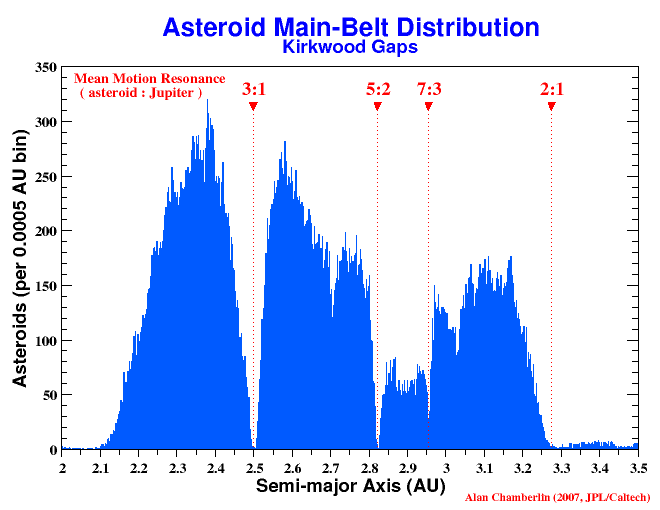
\includegraphics[width=\textwidth]{ast_histo-inverted.png}
\caption{Histogram plot depicting distribution of semi-major axis of 156,929 main-belt asteroids, created in June 2007 \cite{jpl_asteroid_web}.}
\label{fig:mbo_distribution}
\end{figure}
%

Asteroids don't only exist as single bodies in the Solar System, but they are also found in local multi-body systems consisting of two to even three asteroids. With advanced asteroid detection methods, astrophysicists have found over 190 multiple asteroid systems in the Solar System \cite{multipleAsteroids}. Contrary to intuition, these multiple asteroid systems exhibit a wide diversity in terms of the size ratios of the components, their mutual orbits and separation, implicating that the individual components evolved differently over time \cite{multipleAsteroids}. If a multi-asteroid system consists of two or three components, which are bound gravitationally, then it is termed as \textit{binary asteroids} or \textit{triple asteroids} respectively. Triple asteroids are also sometimes termed as \textit{trinary} or \textit{ternary} \cite{multipleAsteroidsTerminology}. Asteroid components that are not gravitationally bound but are genetically related, are termed as \textit{asteroid pairs}. Asteroid pairs where the larger asteroid is a binary or a triple asteroid, are termed as \textit{paired binaries} or \textit{paired triples}, respectively. The larger component in a binary or triple asteroid system or an asteroid pair, is referred to as the \textit{primary} and similarly the smaller component is referred to as the \textit{secondary} \cite{multipleAsteroidsTerminology}. Asteroids are further classified based on their dimensions and thermal properties, for which the reader should read the publication in \cite{multipleAsteroids}.

We now know what asteroids are and the different ways in which they are found in our Solar System, but is it important to study them? There are three major, and most commonly expressed, reasons to study asteroids in our solar system, and not just from a distance such as through radar telescopes placed on Earth, but also through in-situ exploration involving spacecrafts and surface probes. These reasons are mentioned as follows.
\begin{itemize}
\item Asteroids are basically the material left-over from formation of planets in our Solar System. Thus, they are the perfect source to study and understand the origins of the Solar System, as they have remained in the same pristine form since the birth of the Solar System, unlike the planets which have undergone massive topographical and atmospheric changes after their formation. The asteroids can provide valuable information on the chemical composition and initial conditions which led to the formation of planets, including Earth some 4.6 billion years ago. Several scientists have also hypothesized that water and life could have been brought about on Earth through an asteroid or comet and hence exploration of these small bodies could provide a definite answer to an age old question of how life began on Earth \cite{whyAsteroidsWeb}.
\item Asteroids have been hypothesized to have brought complex molecules to the surface of Earth that eventually resulted in life, but lately they have also been linked to the extinction of dinosaurs due to its impact with Earth. Earth is continuously bombarded with very small interplanetary material, most of which doesn't reach the surface of the Earth but gets evaporated in its atmosphere. However, every few 100 years, an asteroid spanning some tens of meter could impact Earth resulting in widespread damage, in the present case to life and property. But the impact from those will not cause the human race to extinct. But every 100,000 years or so, larger asteroids, spanning over tens of kilometer would impact the Earth, which will lead to extinction of life as we know it now. Although the probability of getting hit by an asteroid on such a large scale is low, it is still a statistical possibility and to be able to device strategies for active deflection of such asteroids, it is imperative that we understand more of the dynamics, properties and composition of the asteroids \cite{whyAsteroidsWeb}.
\item The third most important reason for us to study asteroids, is the fact that these small bodies are rich in raw materials or minerals. \gls{NEA} can be exploited for the resources that they possess and use it to build space structures or generate fuel for spacecrafts to enable human space exploration in farther reaches of the Solar System. By studying the asteroids, we can develop methods to tap the vast reservoirs of raw materials residing in them \cite{whyAsteroidsWeb}.
\end{itemize}

\section{Research problem}
In the previous section, we discussed what asteroids are and why its important to study them. In this section, we shall discuss, albeit broadly, the areas of research for the upcoming thesis work. The motivation for this literature study and the future thesis work arises from the fact that past in-situ space exploration activities have made use of explosive capsules to extract subsurface samples for analysis \cite{hayabusa2}. For asteroids with surface made of unconsolidated rock material or dust, use of explosive payloads to expose subsurface material could potentially result in the regolith being lofted from the surface of the asteroid. The lofted material could enter into a long term orbit, or a short term orbit concluding in re-impact of the lofted regolith back on the surface of the asteroid, or even escape the gravitational influence of the asteroid. This idea is fueled by a research paper \cite{idaEjectaErosion} which discusses the re-accretion and and escape of ejecta due to impact from impacts in the Ida system in the main-belt. The lofted regolith poses a serious threat to the safety of the spacecraft in orbit around the asteroid. To avoid any damage to it, it is necessary to develop models that can simulate the motion of the lofted regolith for a given asteroid, to as high an accuracy as possible, so that the mission design for asteroid exploration can account for it and ensure safety of the spacecraft. To do so we need to model the dynamics of the asteroid around the Sun, model the dynamical environment around the asteroid itself, and, although not limited to but also model the dynamics for multiple debris particles lofted from the asteroids surface and account for different perturbing forces that could affect the orbital motion of these particles. By running these simulation models we can compute trajectories for multiple particles at the same time and observe their long or short term behavior.

The tentative research questions shall be presented shortly. We say tentative because in the beginning, the report was aimed to focus on \textit{orbital motion of spacecraft around a binary asteroid system}. However, towards the period around which the report was being concluded, a thesis opportunity was offered from the \gls{CCAR} because of which the thesis topic was changed to \textit{orbital motion of regolith lofted from the surface of an asteroid}. The content of the report is nevertheless useful since it still discusses the dynamics around an asteroid with the difference that instead of a spacecraft, now it will be applied to lofted regolith material. Due to the sudden shift in the focus of the thesis at the time of writing this report, the research questions presented below should be considered as only tentative. The final research questions or problem statements will be mentioned in the final thesis report. The core questions are listed as follows:
\begin{itemize}
\item Simulate, observe and characterize the motion of regolith lofted from the surface of an asteroid for extended periods of time.
\item Does the lofted regolith enter a stable or unstable orbit? What are the corresponding initial conditions and can they be generalized for different asteroids?
\item What is the correlation, if any, between the size of the lofted material against stable or unstable orbital motion? Can a critical size for the lofted material be determined, for the asteroid under study, which would differentiate between stable and unstable orbital motion for the lofted material?
\item In case of stable orbits, are the orbits planar or spatial periodic?
\item In case of an unstable orbit, does the lofted regolith fall back to the surface of the asteroid or does it escape the gravitational influence of the asteroid? Can this behavior be also generalized for a different asteroid?
\item What is the subsequent motion of the regolith that re-impacts on the surface of the asteroid?
\item For a regolith sample return mission based on a touch-and-go technique (such as the \gls{OSIRIS-REx} mission), is it possible to retrieve a sample without causing adjacent surface material to be lofted in to an orbit around the asteroid?
\item For a subsurface sample return mission involving surface detonation (such as the Hayabusa-2 mission), how can the dangers of spacecraft damage from lofted regolith be averted or avoided?
\end{itemize}

\section{Outline of the report}
This literature study report tackles the problem of modeling particle dynamics and solving it in a systematic way. We begin by first describing the various missions that have been to asteroids in the past or are being operated currently along with missions planned for the future in \Cref{heritage}. \Cref{gravpot} discusses the various gravitational potential models that exist and have been applied in past for theoretical studies on orbital mechanics of or around asteroids along with the advantages and disadvantages of each model. \Cref{perturb} presents the relevant orbit perturbation models for working with particle dynamics around asteroids. \Cref{F2BP} begins with a brief introduction to relatively low-fidelity full two-body problem models that have been extensively applied in the past following which an extensive discussion on mutual potential and coupled equations of motion for binary polyhedron-based asteroids is presented. \Cref{RF3BP} begins by introducing the relatively low-fidelity restricted three-body problem but the chapter focuses more on the dynamics of a particle around binary asteroid modeled as two polyhedrons. A linearization technique to reduce simulation loads has also been introduced in that chapter. \Cref{integ} describes and compares the various numerical integration methods; an integrator is needed to propagate the orbital motion of a particle around an asteroid. \Cref{MCS} briefly describes the Monte Carlo simulation technique which will be utilized in our simulation package to generate multiple debris particles at the surface of an asteroid. \Cref{DST} presents some basic concepts on dynamical systems theory such as poincar\'e maps which are used when one wants to characterize the motion of an orbiting particle. And finally, \Cref{conclusion} concludes the literature study report.

\chapter{Results}
\label{results}
\graphicspath{{Results/Images/}}

\section{Regolith launched from the longest edge of the asteroid}
\label{regolith_longest_edge}
The results that we'll discuss in this section pertain to the case of regolith launched from the longest edge of the asteroid, modeled as an ellipsoid.

\subsection{Dynamics without Solar perturbations}
\label{regolith_longest_edge_without_solar}
...to be added later...

\subsection{Dynamics with Solar perturbations}
\label{regolith_longest_edge_with_solar}
In this case, the simulation accounted for perturbations from the irregular gravity field of the asteroid, the \gls{SRP}, and the \gls{STBE}. Within this category, there are 4 distinct sets of simulations, each for a particle with different Area-to-Mass ratio. These are mentioned in \Cref{tab:area_to_mass_ratio}. The material with a density of 3.2 [g/cm$^3$] is low-density Olivine and the one with 7.5 [g/cm$^3$] is Iron-Nickel alloy \cite{passiveSorting}. The mineral Olivine can be found on asteroids and has been discovered on asteroid Itokawa through transmission electron microscope analysis of samples returned by the Hayabusa spacecraft \cite{olivineHayabusa}. Iron-Nickel alloy is found to be most abundant in metallic meteorites \cite{ironAlloy}.
%%%
\begin{table}[]
\centering
\captionsetup{justification=centering}
\caption{Particle Area-to-Mass ratios}
\label{tab:area_to_mass_ratio}
\begin{tabular}{|l|c|c|c|}
\hline
Code    & \multicolumn{1}{l|}{Particle radius {[}cm{]}} & \multicolumn{1}{l|}{Density {[}g/cm$^3${]}} & \multicolumn{1}{l|}{Area-to-Mass ratio {[}m$^2$/kg{]}} \\ \hline
LoGSP-1     &   1.0     &   3.2     &   0.0234      \\ \hline
LoGSP-2     &   1.0     &   7.5     &   0.01        \\ \hline
LoGSP-3     &   5.0     &   3.2     &   0.0047      \\ \hline
LoGSP-4     &   5.0     &   7.5     &   0.002       \\ \hline
\end{tabular}
\end{table}
%%%

For each of the four types of particles mentioned in \Cref{tab:area_to_mass_ratio}, the initial conditions for lofting the regolith are varied in the same manner. These initial conditions are mentioned as follows. The asteroid revolves around the Sun in an equatorial circular orbit at a distance of 1.0 \gls{AU}. Four different initial Solar phase angles were considered for the simulation – 45.0, 135.0, 225.0 315.0 [deg], to account for the four different quadrants where the Sun could be with respect to the asteroid. For each case in \Cref{tab:area_to_mass_ratio}, a total of 72 particles were launched from the surface of the asteroid, each in a different direction (defined using the launch declination and azimuth angles). The launch declination angle, measured from the zenith, was kept constant at 45.0 [deg] for all the particles. The launch azimuth, measured \gls{CCW} from the direction pointing to north, was varied at a resolution of 5.0 [deg] starting from 0.0 [deg] all the way up to 355.0 [deg]. Each particle was launched, in their specified direction, with different velocities ranging from 1.0 [m/s] to 16.0 [m/s] (measured with respect to the asteroid-centric rotating frame) at a resolution of 1.0 [m/s]. So basically, every combination of an initial Solar phase angle, initial launch azimuth, and initial launch velocity corresponds to a unique trajectory for a single particle of a given Area-to-Mass ratio; Thus amounting to a total of 4608 unique trajectories. The simulations were subjected to run for a maximum of 270.0 [days] and were terminated earlier if a particular trajectory resulted in escape or surface re-impact.

\subsubsection{Case LoGSP-1}
\label{LoGSP-1}
The density of the regolith was considered to be 3.2 [g/cm$^{3}$] with a spherical shape of radius 1.0 [cm]. \Cref{fig:LoGSP_1_final_fate_histogram} gives a distribution of particles for each of the three different final fates for the regolith i.e. capture, re-impact, and escape, for different initial launch velocities and initial Solar phase angles. Irrespective of the initial Solar phase, initial launch velocities from 1.0 to 3.0 [m/s] results in particles launched in all directions to eventually re-impact the asteroid's surface. Similarly, for initial launch velocities ranging from 14.0 to 16.0 [m/s], we see that the particles always manage to escape the gravitational attraction of the asteroid. However, there is one exception to the former statement, a single particle launched with a velocity of 14.0 [m/s] at a launch azimuth of 90.0 [deg] and at an initial Solar phase angle of 315.0 [deg], re-impacts the asteroid's surface. It is interesting to note that the launch azimuth of the particle is such that it is launched in a direction that is directly opposite to the direction of rotation of the asteroid. Launch velocities from 4.0 to 13.0 [m/s] show a mixed behavior and the final fate distribution trend does not vary drastically for different initial Solar phase angles.

The number of capture cases is far less than those for escape and re-impact. For initial Solar phase of 225.0 [deg], there are no cases of regolith being captured in orbit around the asteroid. All capture cases, arranged in order of increasing launch azimuth angle, are listed in \Cref{tab:LoGSP_1_capture}. It is interesting to note that all capture cases result from when the particle is launched in a direction which is against the direction of rotation of the asteroid, bar one exception which is case index-11 in \Cref{tab:LoGSP_1_capture}.
%%%
\begin{table}[htb]
\centering
\captionsetup{justification=centering}
\caption{Initial conditions that resulted in temporary orbital capture of regolith around the asteroid. Particle code LoGSP-1.}
\label{tab:LoGSP_1_capture}
\begin{tabular}{|l|c|c|c|}
\hline
Index & \multicolumn{1}{l|}{Launch azimuth [deg]} & \multicolumn{1}{l|}{Launch velocity [m/s]} & \multicolumn{1}{l|}{Initial Solar phase angle [deg]} \\ \hline
\rowcolor[HTML]{FE996B}
1   & 5.0 & 5.0 & 315.0     \\ \hline
\rowcolor[HTML]{67FD9A}
2   & 10.0 & 9.0 & 135.0    \\ \hline
\rowcolor[HTML]{9698ED}
3   & 15.0 & 8.0 & 45.0     \\ \hline
\rowcolor[HTML]{FFCC67}
4   & 45.0 & 12.0 & 45.0    \\ \hline
\rowcolor[HTML]{96FFFB}
5   & 45.0 & 10.0 & 315.0   \\ \hline
\rowcolor[HTML]{FFCC67}
6   & 135.0 & 12.0 & 45.0   \\ \hline
\rowcolor[HTML]{96FFFB}
7   & 135.0 & 10.0 & 315.0  \\ \hline
\rowcolor[HTML]{9698ED}
8   & 165.0 & 8.0 & 45.0    \\ \hline
\rowcolor[HTML]{67FD9A}
9   & 170.0 & 9.0 & 135.0   \\ \hline
\rowcolor[HTML]{FE996B}
10  & 175.0 & 5.0 & 315.0   \\ \hline
11  & 185.0 & 5.0 & 135.0   \\ \hline
\end{tabular}
\end{table}
%%%
The capture cases which represent symmetry in terms of the launch azimuth angle are highlighted with the same color in \Cref{tab:LoGSP_1_capture}. This symmetric behavior results from the combination of two factors. First, the Sun's motion relative to the asteroid is not in an inclined plane, and secondly, the particles are launched from the equatorial tip of the ellipsoid shaped asteroid, which is a point of symmetry on the ellipsoid. The capture cases will be discussed in detail a bit further ahead.
%%%
\begin{figure}[htb]
\centering
\captionsetup{justification=centering}
% another option for includegraphics - keepaspectratio
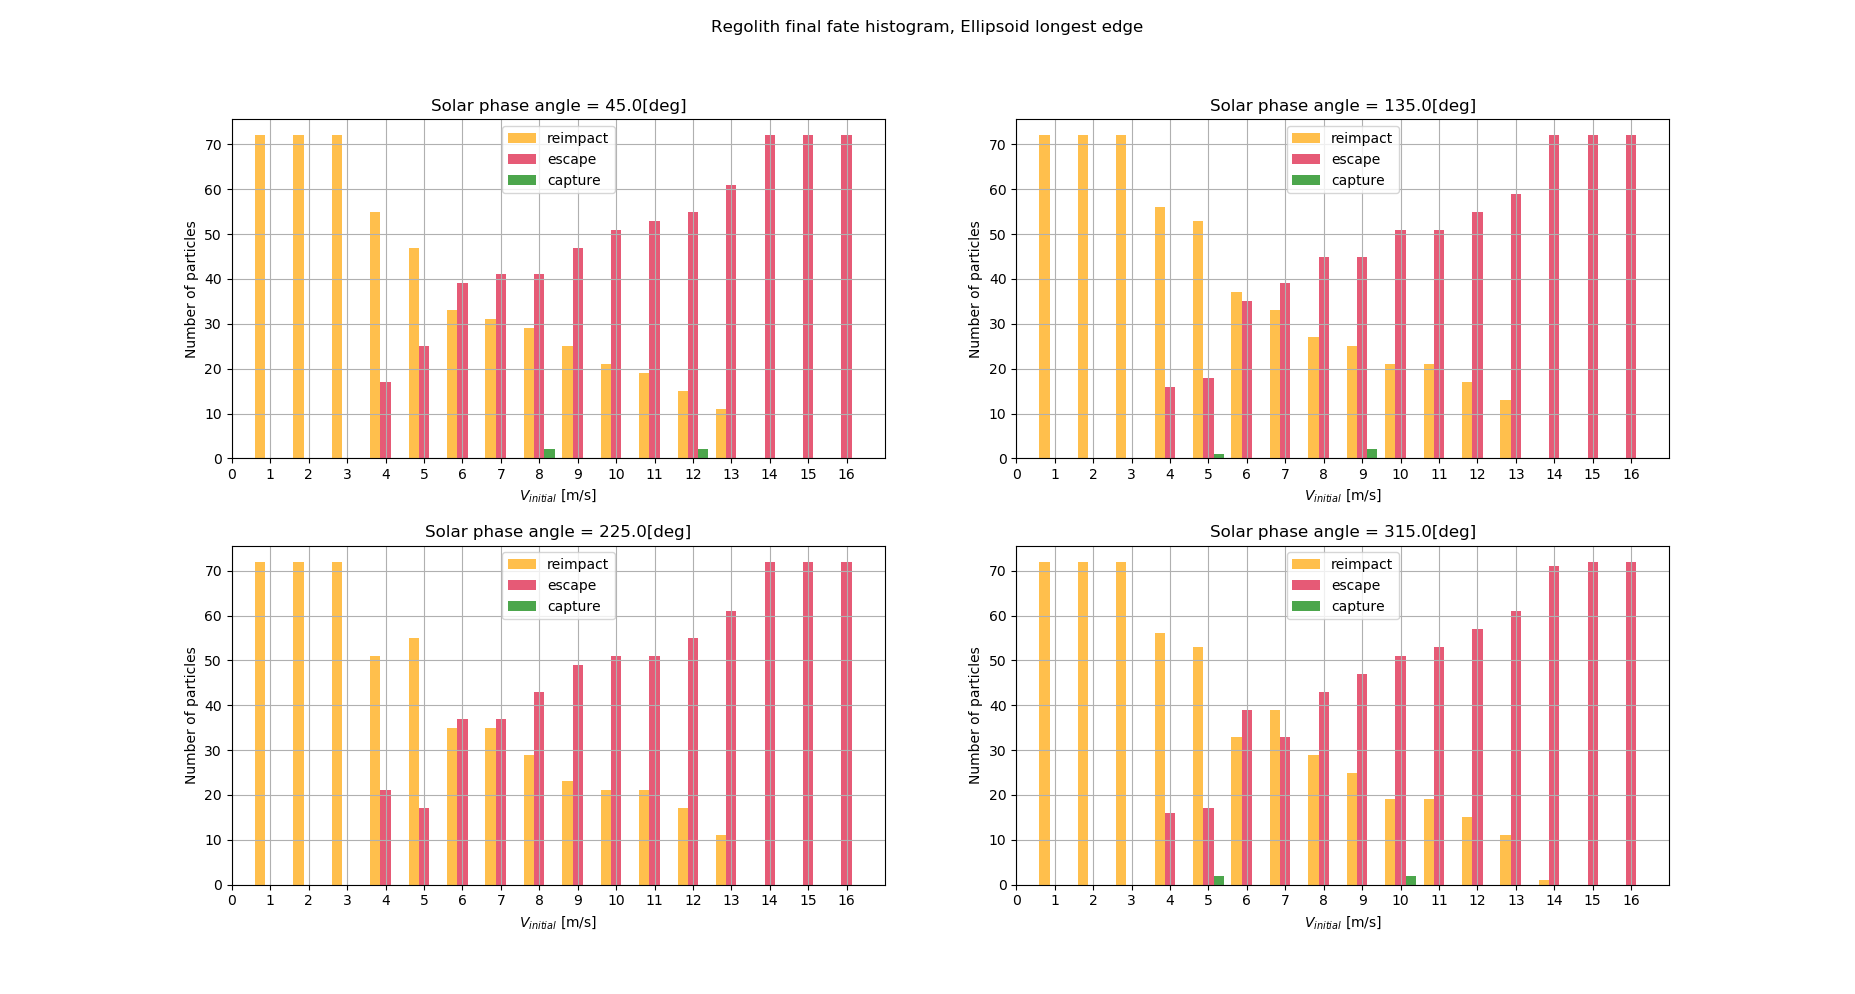
\includegraphics[angle=90, width=\textwidth, height=\textheight]{longest_edge_perturbations/3.2Density_1cmSize/final_fate_versus_launch_velocity_histogram_all_solar_phases.png}
\caption{Histogram showing the number of particles that re-impact, escape, or get captured around the asteroid, for different initial launch velocities. Particle code LoGSP-1.}
\label{fig:LoGSP_1_final_fate_histogram}
\end{figure}
\FloatBarrier
%%%
\Cref{fig:LoGSP_1_crashmap} depicts the surface distribution of regolith that re-impacts the surface when launched from the same location with different velocities and different initial Solar phase angles. The launch location is in the centre of the map, Latitude 0.0 [deg] and Longitude 0.0 [deg]. The particle distribution is the same for regions close to the launch point and for lower launch velocities up until 8.0 [m/s]. A similarity in distribution pattern is also observed around Longitude -150.0 [deg] for launch velocity of 9.0 [m/s] and around Longitude 150.0 [deg] for launch velocity of 10.0 [m/s] for the four Solar phase angles. The distribution pattern, for all launch velocities and initial Solar phases, is also symmetric about the equator. Again, the reason for this is the same as mentioned earlier for the symmetry in capture cases in \Cref{tab:LoGSP_1_capture}. Keeping the launch direction and velocity constant, we see that the distribution of regolith that re-impacts the surface does not change drastically with varying initial Solar phase angles, except for a relatively few cases. This is much easily observed in a plot of Range from the launch direction to the re-impact point versus launch azimuth for different velocities as shown in \Cref{fig:LoGSP_1_range_comparison}.

We haven't shown the range to re-impact point plots in \Cref{fig:LoGSP_1_range_comparison} for all launch velocities because the intention here is to show the qualitative behavior, which can be achieved by considering only a subset of the launch velocities that result in a re-impact scenario. The very first thing we observe is that as the launch velocity increases, the range of launch azimuth over which the regolith re-impacts the surface reduces because a higher velocity allows the regolith to enter a higher orbit (as it attains a relatively higher energy) and reduces the probability of a re-impact. Even as the velocity increases, we see that the azimuths that result in a re-impact are the ones in which the regolith is launched in a direction that is opposite to the asteroid's rotation direction. This makes sense since the regolith's energy would be reduced the most in this scenario compared to all other launch directions, thereby increasing the chances of a re-impact.

Now the primary purpose of the plots in \Cref{fig:LoGSP_1_range_comparison} (combined with \Cref{fig:LoGSP_1_crashmap}) is to depict the qualitative effect of Solar perturbations, for varying initial Solar phase angles, on the re-impact behavior of regolith compared to the case when no Solar perturbations are considered. For launch velocities of 4.0, 7.0 and 10.0 [m/s], we see that the Solar perturbations do not affect the re-impact location for cases when the particle is launched in directions opposite to that of the asteroid's rotation. However, we do see few exceptions to the former statement, most noticeably in the case of 7.0 [m/s]. But for the majority of cases where the re-impact location remains unchanged, we see from \Cref{fig:LoGSP_1_reimpact_time}, that these particles spend less than 3.0 [Hrs] in orbit which is not enough time for the Solar perturbations to act and have any significant impact on the dynamics of the particles. So in essence this is what's happening here - Particles when launched in a direction that is opposite to that of the asteroid's rotation, even at relatively high velocities such as 10.0 [m/s], loose enough energy to stay in a relatively lower orbit (see \Cref{fig:LoGSP_1_maxAltitude_reimpactscenario}) where the gravitational force of the asteroid is significantly stronger than any of the Solar perturbations and as the particle spends a very short time in orbit before re-impact, the Solar perturbations do not get enough time to affect the particle's orbit and hence the particle re-impacts the same location as it would have when no Solar perturbations were considered in the simulation. For the lower launch velocities of 4.0 and 7.0 [m/s], the differences in re-impact locations are more pronounced when the regolith is launched in the same direction as that of the asteroid's rotation. Particles gain relatively higher energy in this case, enter a higher orbit and spend enough time in there for the Solar perturbations to affect it's motion. For the case of the launch velocity of 13.0 [m/s] in \Cref{fig:LoGSP_1_range_comparison}, the velocity is high enough such that the particle does not loose enough energy when launched opposite to the asteroid's rotational direction and is able to enter a relatively higher orbit (see \Cref{fig:LoGSP_1_maxAltitude_reimpactscenario}) and stay there for a relatively longer time, as seen in \Cref{fig:LoGSP_1_reimpact_time}, which results in the Solar perturbations affecting the orbital motion and eventually the re-impact location of the regolith.
%%%
\begin{figure}[htb]
\centering
\captionsetup{justification=centering}
% another option for includegraphics - keepaspectratio
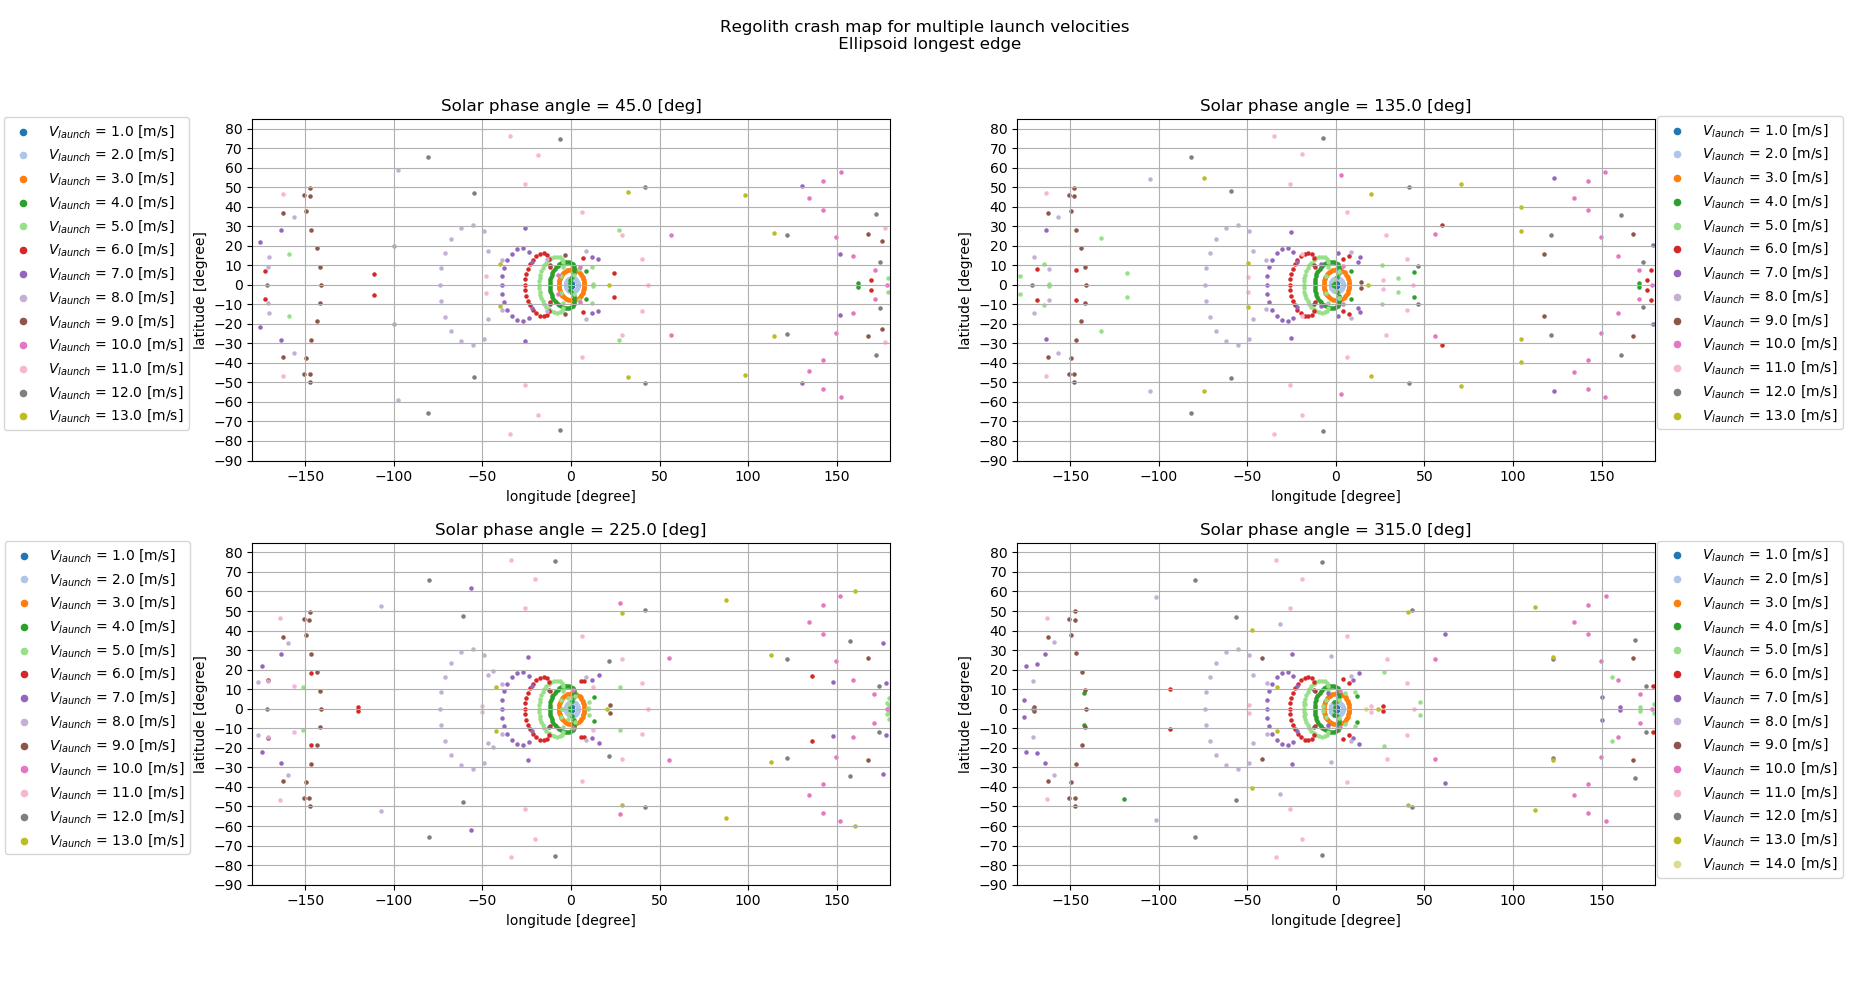
\includegraphics[angle=90, width=\textwidth, height=\textheight]{longest_edge_perturbations/3.2Density_1cmSize/crash_map_all_solar_phases.png}
\caption{Surface distribution of re-impacted regolith for different launch velocities. The launch location is \\ latitude: 0.0 [deg], longitude: 0.0 [deg]. Particle code LoGSP-1.}
\label{fig:LoGSP_1_crashmap}
\end{figure}
\FloatBarrier
%%%
%%%
\begin{figure}[htb]
\centering
\captionsetup{justification=centering}
% another option for includegraphics - keepaspectratio
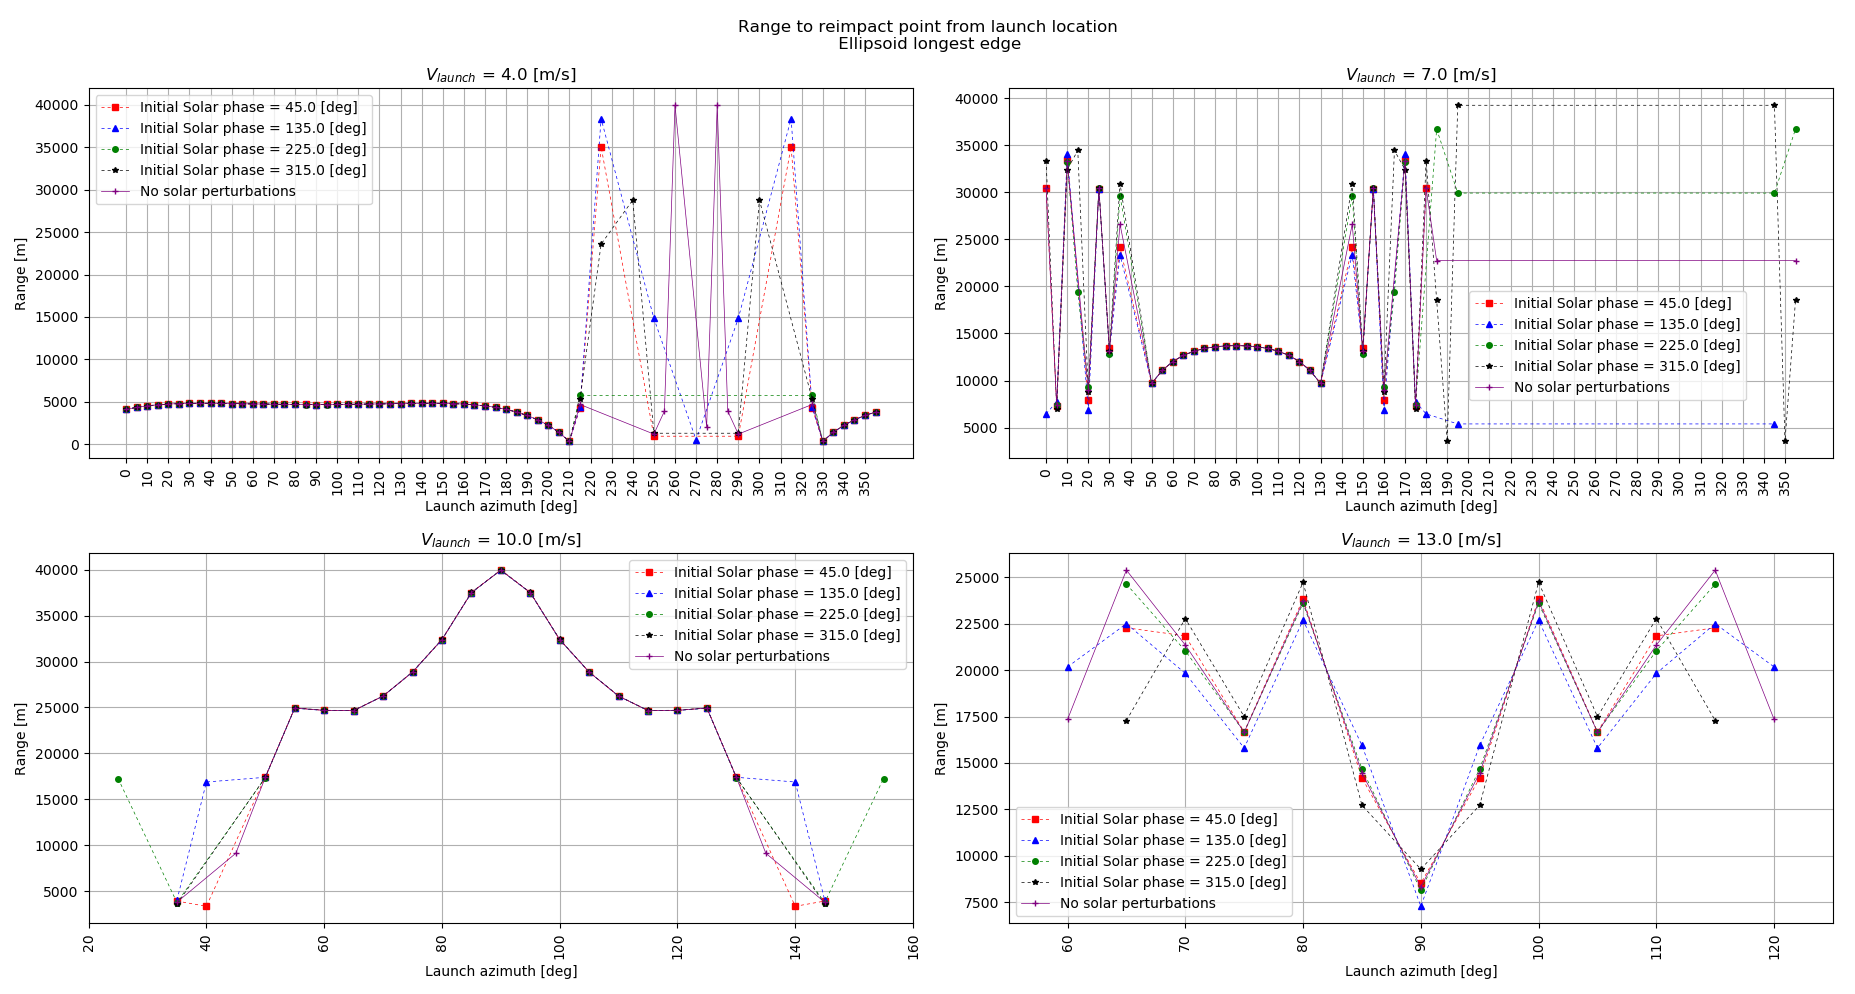
\includegraphics[angle=90, width=\textwidth, height=\textheight]{longest_edge_perturbations/3.2Density_1cmSize/reimpactRangeComparison.png}
\caption{Range to re-impact location from the launch point for different velocities. Particle code LoGSP-1.}
\label{fig:LoGSP_1_range_comparison}
\end{figure}
\FloatBarrier
%%%
%%%
\begin{figure}[htb]
\centering
\captionsetup{justification=centering}
% another option for includegraphics - keepaspectratio
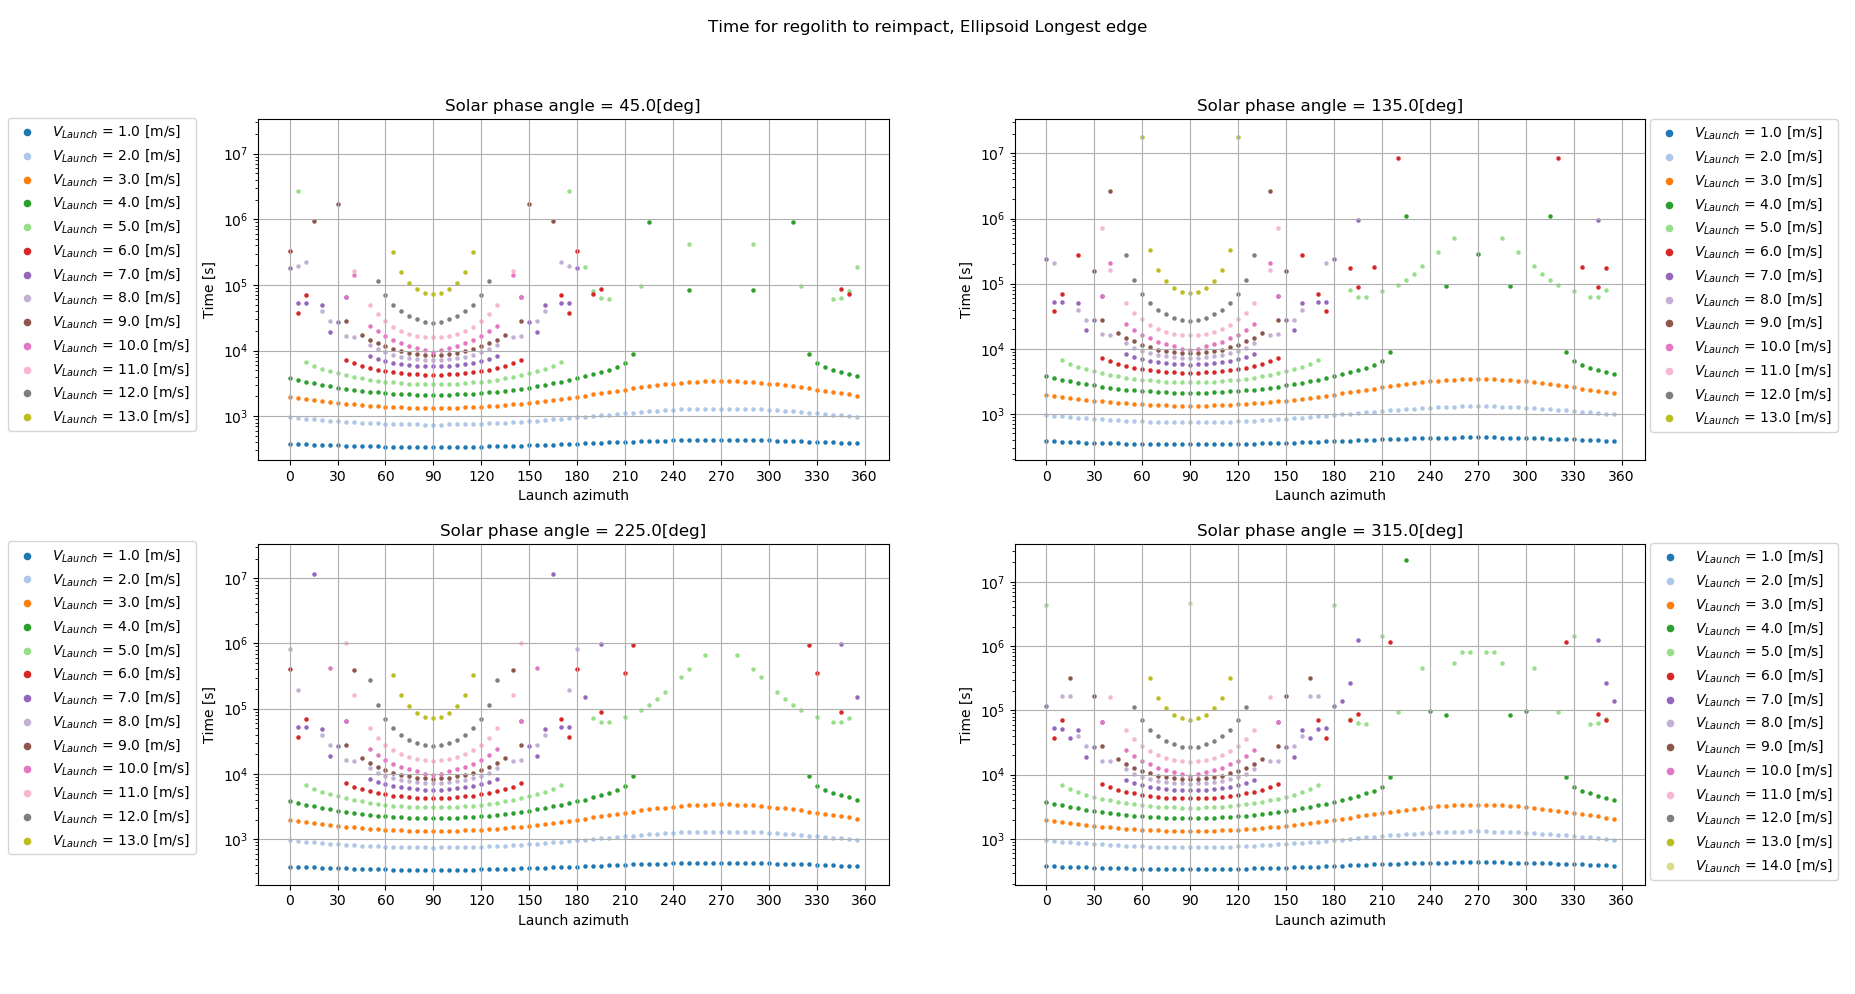
\includegraphics[angle=90, width=\textwidth, height=\textheight]{longest_edge_perturbations/3.2Density_1cmSize/time_to_reimpact_all_solar_phases.png}
\caption{Time taken by regolith at different velocities and launch directions to re-impact with the surface of the asteroid. Particle code LoGSP-1.}
\label{fig:LoGSP_1_reimpact_time}
\end{figure}
\FloatBarrier
%%%
We shall now look at the cases where the lofted regolith gets (temporarily) captured in orbit by the asteroid. The initial conditions for all capture cases, for the current particle size and density, were mentioned earlier in \Cref{tab:LoGSP_1_capture}. \Cref{fig:LoGSP_1_capture_orbital_range} depicts the progression in orbital range of the temporarily captured regolith. The straight lines in the plot are used to mark the different altitude regimes. These are the \gls{LAO}, \gls{MAO}, \gls{HAO}, \gls{UHAO}, and \gls{EHAO}. These altitude regime definitions are not from well defined standards, but instead were arbitrarily chosen as integer multiples of the longest semi-major axis, $\alpha$, of the tri-axial ellipsoid shaped asteroid. The definition for these altitude regimes is given in \Cref{tab:altitude_regimes}.
%%%
\begin{table}[htb]
\centering
\captionsetup{justification=centering}
\caption{Altitude regimes and their definitions}
\label{tab:altitude_regimes}
\begin{tabular}{|c|c|}
\hline
\textbf{Altitude regime}        & \textbf{Definition}                    \\ \hline
\gls{LAO}                       & Asteroid surface to $2 \times \alpha$  \\ \hline
\gls{MAO}                       & $2 \times \alpha$ to $3 \times \alpha$ \\ \hline
\gls{HAO}                       & $3 \times \alpha$ to $5 \times \alpha$ \\ \hline
\gls{UHAO}                      & $5 \times \alpha$ to $7 \times \alpha$ \\ \hline
\gls{EHAO}                      & Above $7 \times \alpha$                \\ \hline
\end{tabular}
\end{table}
\FloatBarrier
%%%
The purpose of plotting data as shown in \Cref{fig:LoGSP_1_capture_orbital_range} was to look for any patterns or periodicity, if they existed, and to see if particles in temporary capture scenario remain closer to the asteroid or further away from it. The symmetry as explained for initial conditions mentioned in \Cref{tab:LoGSP_1_capture} can also be seen in \Cref{fig:LoGSP_1_capture_orbital_range}, for example, regolith launched with velocity of 8.0 [m/s] and launch azimuth of 15.0 [deg] (shown by the purple curve in the top plot in \Cref{fig:LoGSP_1_capture_orbital_range}) shows the same behavior as that of regolith launched with the same velocity and 165.0 [deg] launch azimuth (shown by the green curve in the bottom plot in \Cref{fig:LoGSP_1_capture_orbital_range}). Another thing we see from the plot is that, apart from case number 11 in \Cref{tab:LoGSP_1_capture}, the captured regolith stay in the higher altitude regions for most part and only briefly do they fall within the \gls{MAO} and \gls{LAO} region. We shall now look at atleast three cases from \Cref{fig:LoGSP_1_capture_orbital_range} in a bit more detail to understand the effect of Solar perturbations by comparing these cases with their counterparts from the simulation where Solar perturbations were omitted.

Of all the cases shown in \Cref{fig:LoGSP_1_capture_orbital_range} or \Cref{tab:LoGSP_1_capture}, the one with a launch velocity of 10.0 [m/s] and launch azimuth of 45.0 [deg] results in a re-impact scenario when Solar perturbations are omitted but the same initial conditions lead to a temporary capture orbit when perturbations were added for an initial Solar phase angle of 315.0 [deg]. Every other initial condition for the capture cases had otherwise resulted in an escape situation when simulations were conducted without the Solar perturbations. The 3D trajectory plot in two different views for the former case are shown in \Cref{fig:LoGSP_1_capture_case_5_3d_traj_inertialFrame_differnetViews} (see \Cref{fig:LoGSP_1_capture_case_5_3d_trajectory} also for the 3D trajectory representation in body fixed frame). The 2D trajectory for the same is shown in \Cref{fig:LoGSP_1_capture_case_5_2d_traj_inertialFrame} in inertial frame and in \Cref{fig:LoGSP_1_capture_case_5_2d_traj_bodyFrame} in the asteroid centric rotating frame or the body frame. The web-link or URL for the trajectory animation of the particle (in inertial frame and in XY plane only) can be found in \Cref{fig:LoGSP_1_capture_case_5_2d_trajectory_animation}.
%%%
\begin{figure}[htb]
\centering
\captionsetup{justification=centering}
% another option for includegraphics - keepaspectratio

\includegraphics[scale=0.25]{longest_edge_perturbations/3.2Density_1cmSize/qrcode_10ms_45Azimuth_315SolarPhase.png}
\caption{2D trajectory animation (XY Plane) of capture regolith for case number 5 in \Cref{tab:LoGSP_1_capture}. Particle code LoGSP-1. Scan the QR code to view the animation or use the following web-link: \url{https://youtu.be/oZDhDo5CIsk}}
\label{fig:LoGSP_1_capture_case_5_2d_trajectory_animation}
\end{figure}
\FloatBarrier
%%%
%%%
\begin{figure}[p]
\centering
\captionsetup{justification=centering}
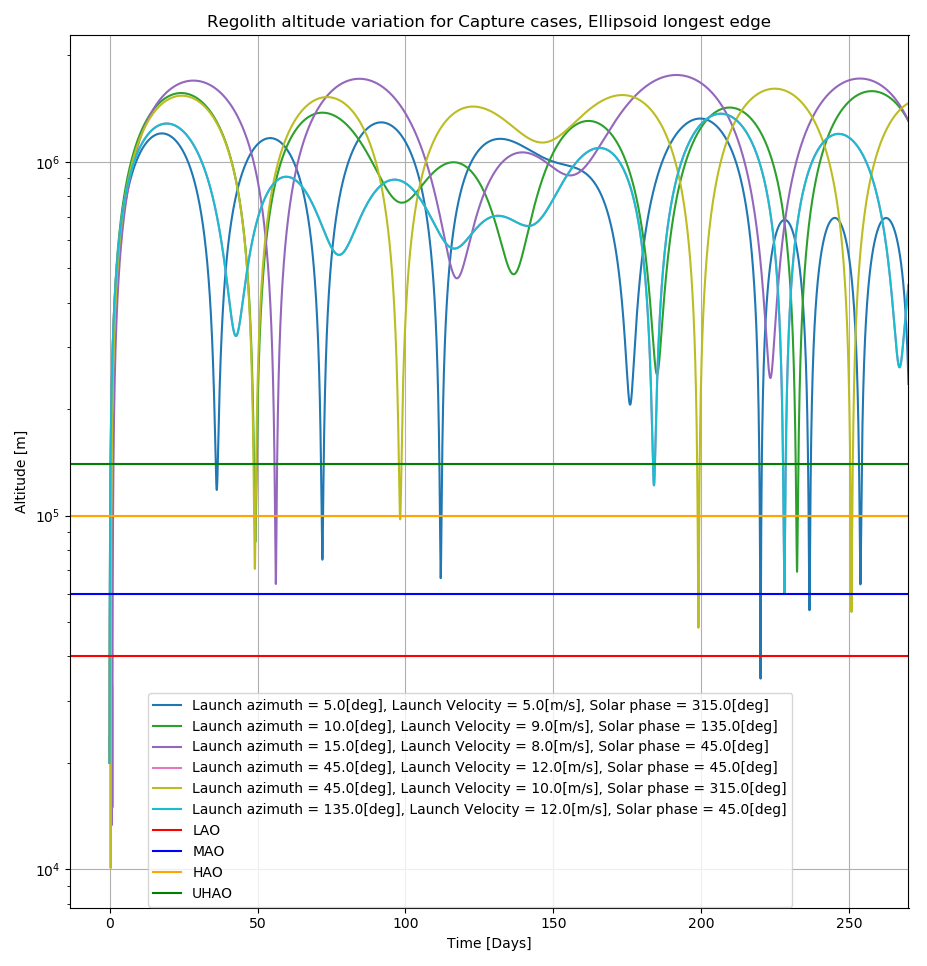
\includegraphics[scale=0.5]{longest_edge_perturbations/3.2Density_1cmSize/altitude_versus_time_all_cases_part_1.png}
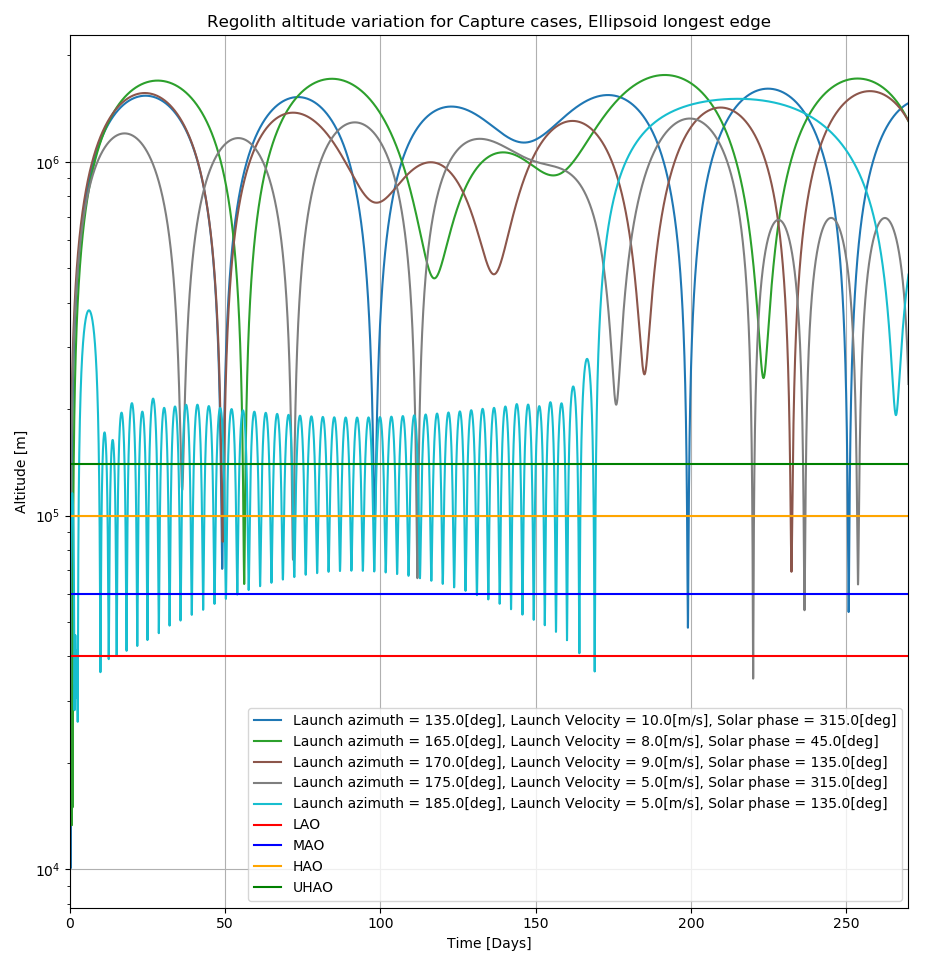
\includegraphics[scale=0.5]{longest_edge_perturbations/3.2Density_1cmSize/altitude_versus_time_all_cases_part_2.png}
\caption{Orbital range progression with time for temporary capture scenarios. Particle code LoGSP-1.}
\label{fig:LoGSP_1_capture_orbital_range}
\end{figure}
\FloatBarrier
%%%
%%%
\begin{figure}[htb]
\centering
\captionsetup{justification=centering}
% another option for includegraphics - keepaspectratio
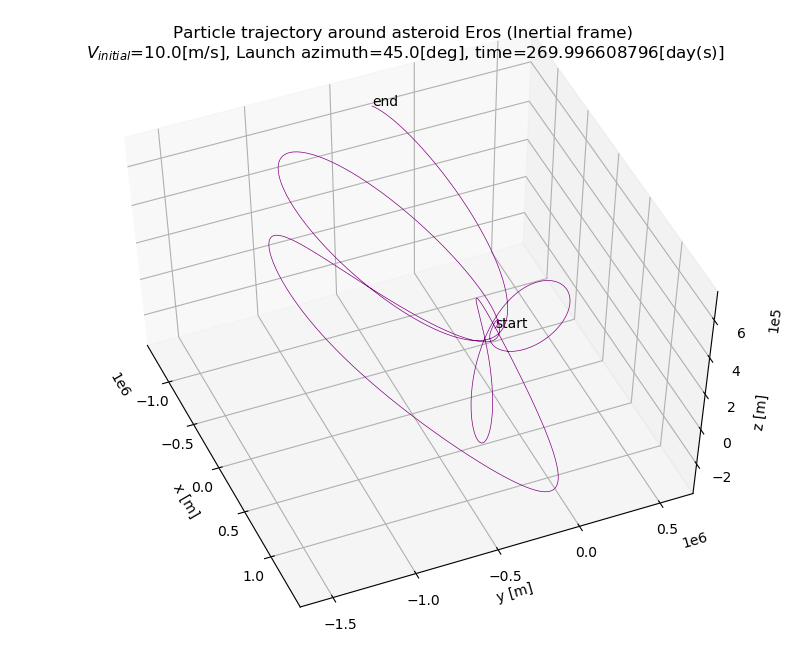
\includegraphics[scale=0.7]{longest_edge_perturbations/3.2Density_1cmSize/3dTrajectory_10ms_45Azimuth_315solarPhase_inertialFrame_View1.png}
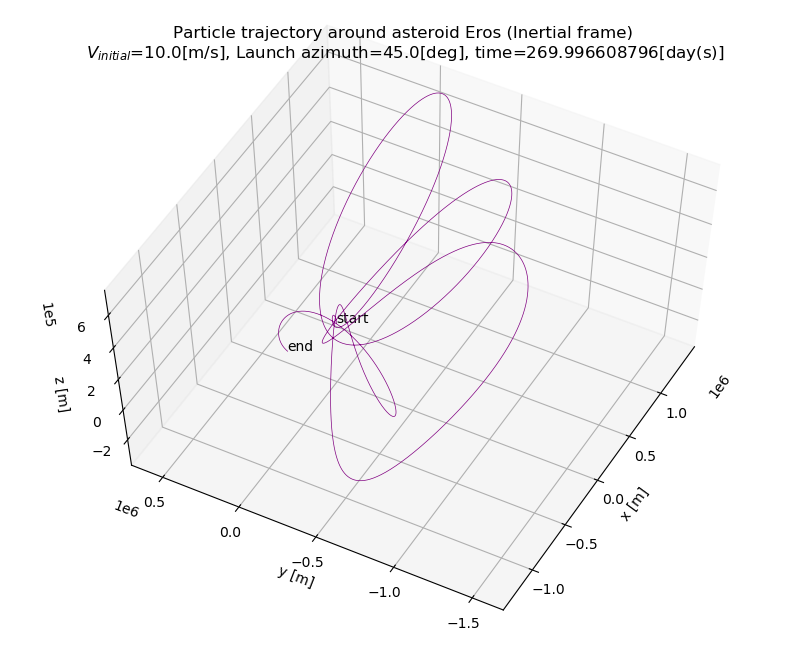
\includegraphics[scale=0.7]{longest_edge_perturbations/3.2Density_1cmSize/3dTrajectory_10ms_45Azimuth_315solarPhase_inertialFrame_View2.png}
\caption{3D inertial frame trajectory of capture regolith for case number 5 in \Cref{tab:LoGSP_1_capture} in two different viewing angles. Particle code LoGSP-1.}
\label{fig:LoGSP_1_capture_case_5_3d_traj_inertialFrame_differnetViews}
\end{figure}
\FloatBarrier
%%%
Note that in the trajectory animation in \Cref{fig:LoGSP_1_capture_case_5_2d_trajectory_animation} (and any other animation included henceforth) the particle is made to skip several data points in between along the trajectory when it is far away from the asteroid, just to reduce the length of the animation. So because of this, the particle appears to be moving faster when it is away from the asteroid but this is not true. For the exact velocity of the particle, the reader should look at the velocity magnitude indicator within the animation itself.

The animation shows that the particle reverses its direction of motion twice in its entire course. To visualize how this is happening in 3D, look at \Cref{fig:LoGSP_1_capture_case_5_3d_traj_inertialFrame_differnetViews}. The reason for this can be understood by looking at the direction of the perturbing vectors in \Cref{fig:LoGSP_1_capture_case_5_2d_trajectory_perturbationVectors}. The plot shows the direction of the perturbing acceleration vector in the XY plane. Both \gls{SRP} and \gls{STBE} are shown separately as well as the net effect of the two. The vectors (in all three plots in \Cref{fig:LoGSP_1_capture_case_5_2d_trajectory_perturbationVectors}) are shown along those parts of the trajectory where the magnitude of \gls{SRP} acceleration is of the same order of magnitude as that of the gravitational acceleration. However, the magnitude of the \gls{STBE} acceleration is always 1.0 order of magnitude smaller than the gravitational acceleration for those very same points along the trajectory. The \gls{SRP} is definitely more dominant of the two Solar perturbations as we can see that the direction of the net perturbation is the same as that of \gls{SRP}. In the plots, the trajectory loops numbered 1 and 2, is where the particle's direction of motion reversed. And this happens because of the \gls{SRP}, as the direction of the perturbation is such that it pulls the particle away from its nominal motion and forces it to change its direction. This is an interesting effect and happens only because the \gls{SRP} offers an acceleration to the particle which is equally significant as the gravitational acceleration when the particle is far away from the asteroid. This is not an isolated incident and we'll show another example where this happens.

\Cref{fig:LoGSP_1_capture_case_8_3d_traj_inertialFrame_differnetViews} shows the 3D trajectory for completely different launch conditions (see capture case 8 in \Cref{tab:LoGSP_1_capture}). The 3D trajectory as viewed from the asteroid centric body fixed frame is shown in \Cref{fig:LoGSP_1_capture_case_8_3d_trajectory}. The 2D trajectory projections for the same, in inertial and body fixed frames, are shown in \Cref{fig:LoGSP_1_capture_case_8_2d_traj_inertialFrame} and \Cref{fig:LoGSP_1_capture_case_8_2d_traj_bodyFrame} respectively. Just like in the previous case, we see from the animation (see \Cref{fig:LoGSP_1_capture_case_8_2d_trajectory_animation}) and the 3D trajectory for current launch conditions that the particle direction of motion is reversed twice in its course. If we look at \Cref{fig:LoGSP_1_capture_case_8_2d_trajectory_perturbationVectors}, we see it again that the change in direction is happening because of the perturbations and more significantly by the \gls{SRP}. The perturbation vectors in \Cref{fig:LoGSP_1_capture_case_8_2d_trajectory_perturbationVectors} are plotted for points along the trajectory where the magnitude of acceleration due to \gls{SRP} is of the same order of magnitude as the gravitational acceleration. Again, the magnitude of \gls{STBE} is 1.0 order of magnitude smaller than the gravitational acceleration for the same data points along the trajectory. Along loops numbered 1 and 2 in \Cref{fig:LoGSP_1_capture_case_8_2d_trajectory_perturbationVectors} the \gls{SRP} direction is such that it forces the particle to change its direction of motion from its nominal course.
%%%
\begin{figure}[htb]
\centering
\captionsetup{justification=centering}
% another option for includegraphics - keepaspectratio

\includegraphics[scale=0.2]{longest_edge_perturbations/3.2Density_1cmSize/qrcode_8ms_165Azimuth_45SolarPhase.png}
\caption{2D trajectory animation (XY Plane) of capture regolith for case number 8 in \Cref{tab:LoGSP_1_capture}. Particle code LoGSP-1. Scan the QR code to view the animation or use the following web-link: \url{https://youtu.be/CceYRlNvAiM}}
\label{fig:LoGSP_1_capture_case_8_2d_trajectory_animation}
\end{figure}
\FloatBarrier
%%%
In both the capture cases that we discussed so far, we can see that out of \gls{SRP} and \gls{STBE}, the former has a more deciding effect on the motion of the particle when it is far away from the asteroid. The way the particles change their direction of motion is consistent with the direction in which the \gls{SRP} perturbation is acting. So now we know how \gls{SRP} is affecting a particle's motion while it is in a capture orbit around an asteroid. But now, we shall take a look at how these Solar perturbations are also responsible for creating a capture orbit in the first place.
%%%
\begin{figure}[htb]
\centering
\captionsetup{justification=centering}
% another option for includegraphics - keepaspectratio
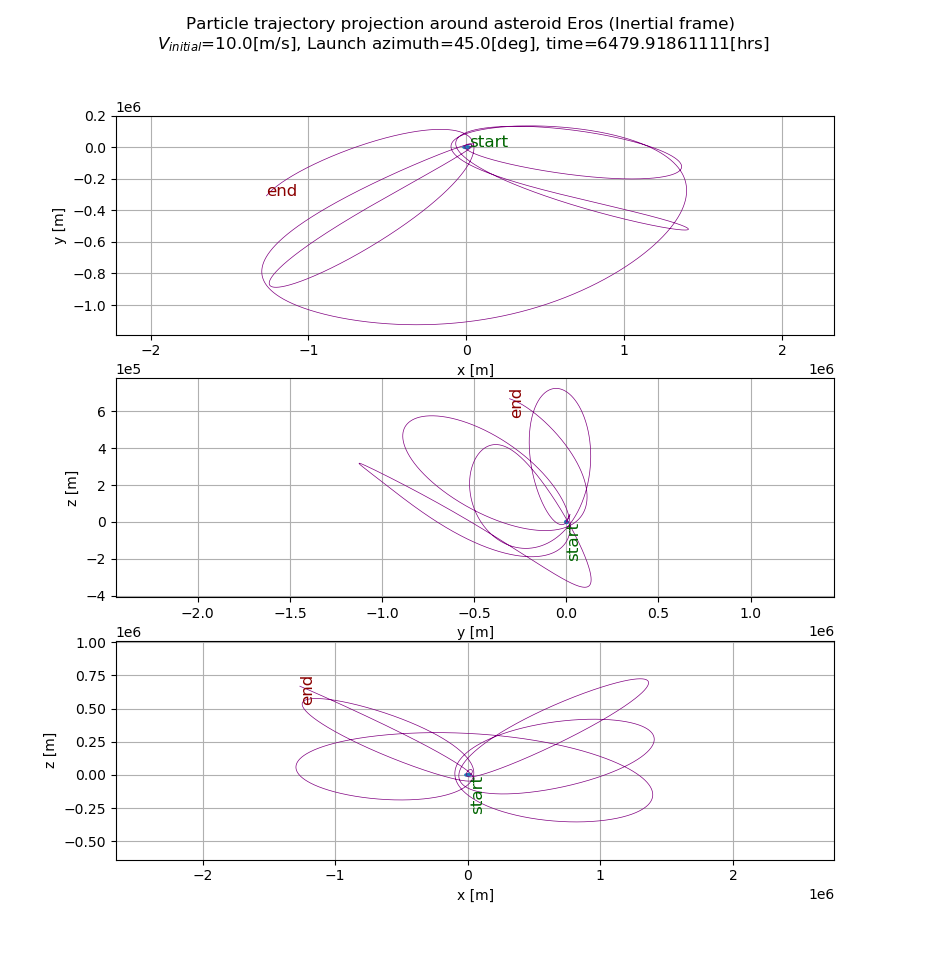
\includegraphics[width=\textwidth, height=\textheight]{longest_edge_perturbations/3.2Density_1cmSize/2dTrajectory_10ms_45Azimuth_315solarPhase_inertialFrame.png}
\caption{2D inertial frame trajectory of capture regolith for case number 5 in \Cref{tab:LoGSP_1_capture}. Particle code LoGSP-1.}
\label{fig:LoGSP_1_capture_case_5_2d_traj_inertialFrame}
\end{figure}
\FloatBarrier
%%%
\begin{figure}[htb]
\centering
\captionsetup{justification=centering}
% another option for includegraphics - keepaspectratio
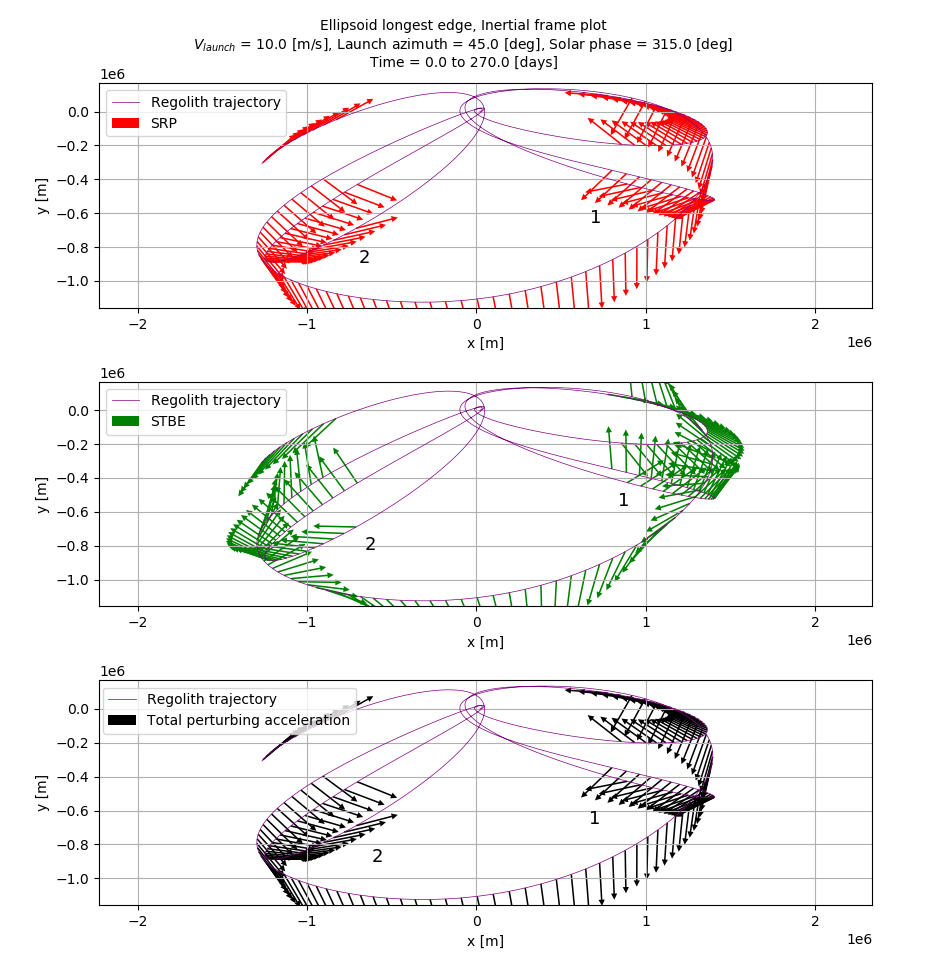
\includegraphics[width=\textwidth, height=\textheight]{longest_edge_perturbations/3.2Density_1cmSize/TotalPerturbingVector_xyPlane_completeTraj_10ms_45DegAzim_315SolarPhase_edit.png}
\caption{2D trajectory of capture regolith for case number 5 in \Cref{tab:LoGSP_1_capture} with direction of \gls{SRP} and \gls{STBE} perturbation vectors along with the sum total of the two. Note that the vectors are shown only for those parts of the trajectory where the \gls{SRP} magnitude is of the same order as that of the asteroid's gravitational acceleration. For those very same points along the trajectory, the magnitude of the \gls{STBE} is always 1.0 order of magnitude smaller than the gravitational acceleration. Particle code LoGSP-1.}
\label{fig:LoGSP_1_capture_case_5_2d_trajectory_perturbationVectors}
\end{figure}
\FloatBarrier
%%%
%%%
\begin{figure}[htb]
\centering
\captionsetup{justification=centering}
% another option for includegraphics - keepaspectratio
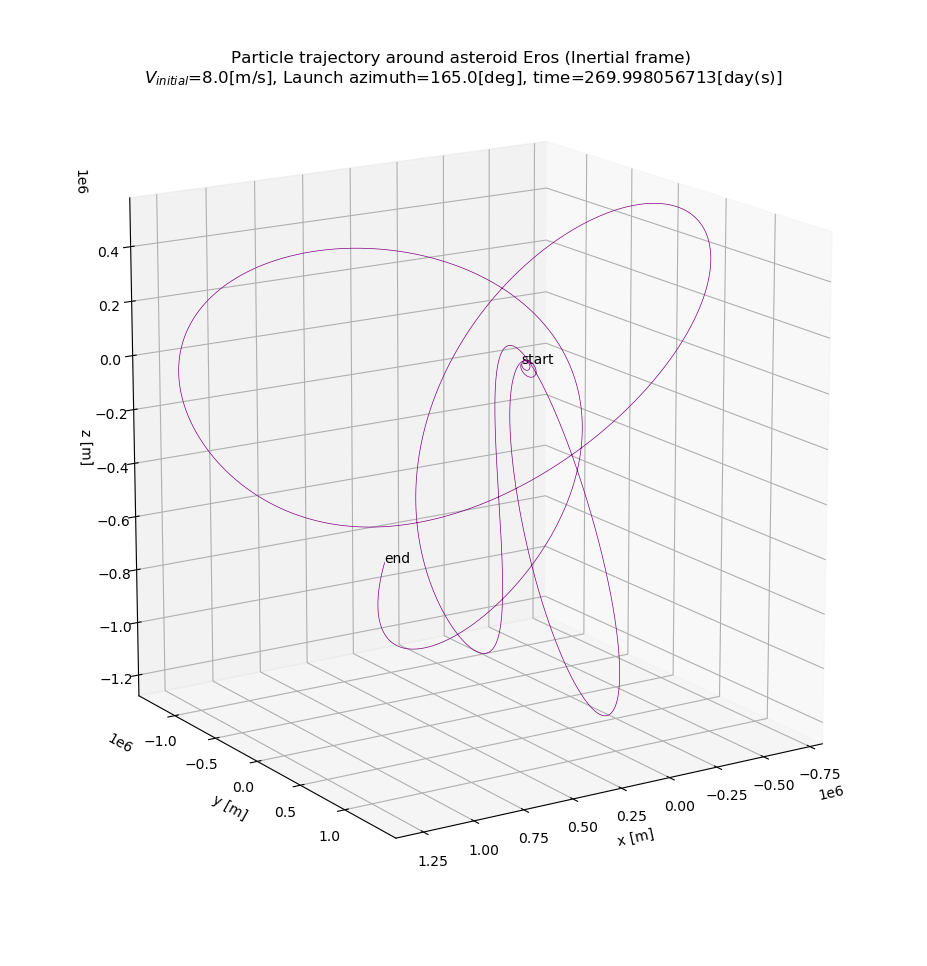
\includegraphics[scale=0.50]{longest_edge_perturbations/3.2Density_1cmSize/3dTrajectory_8ms_165Azimuth_45solarPhase_View3.png}
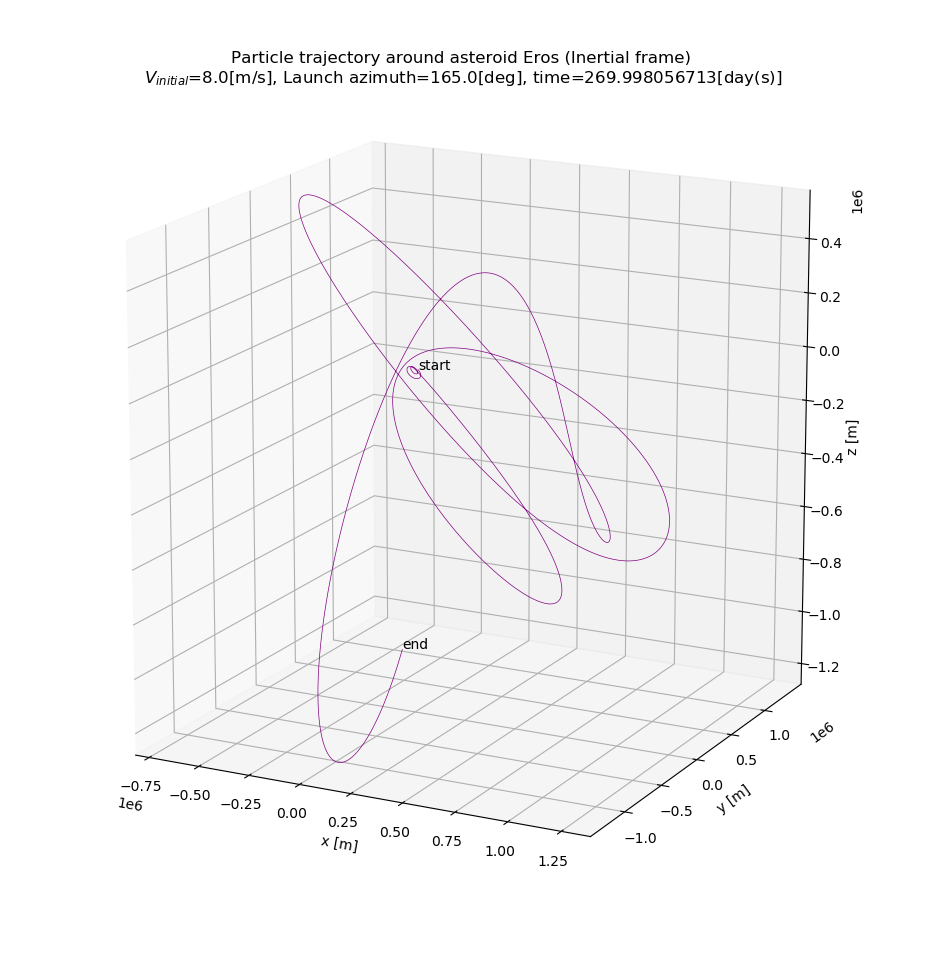
\includegraphics[scale=0.50]{longest_edge_perturbations/3.2Density_1cmSize/3dTrajectory_8ms_165Azimuth_45solarPhase_View4.png}
\caption{3D inertial frame trajectory of capture regolith for case number 8 in \Cref{tab:LoGSP_1_capture} from two different viewing angles. Particle code LoGSP-1.}
\label{fig:LoGSP_1_capture_case_8_3d_traj_inertialFrame_differnetViews}
\end{figure}
\FloatBarrier
%%%
%%%
\begin{figure}[htb]
\centering
\captionsetup{justification=centering}
% another option for includegraphics - keepaspectratio
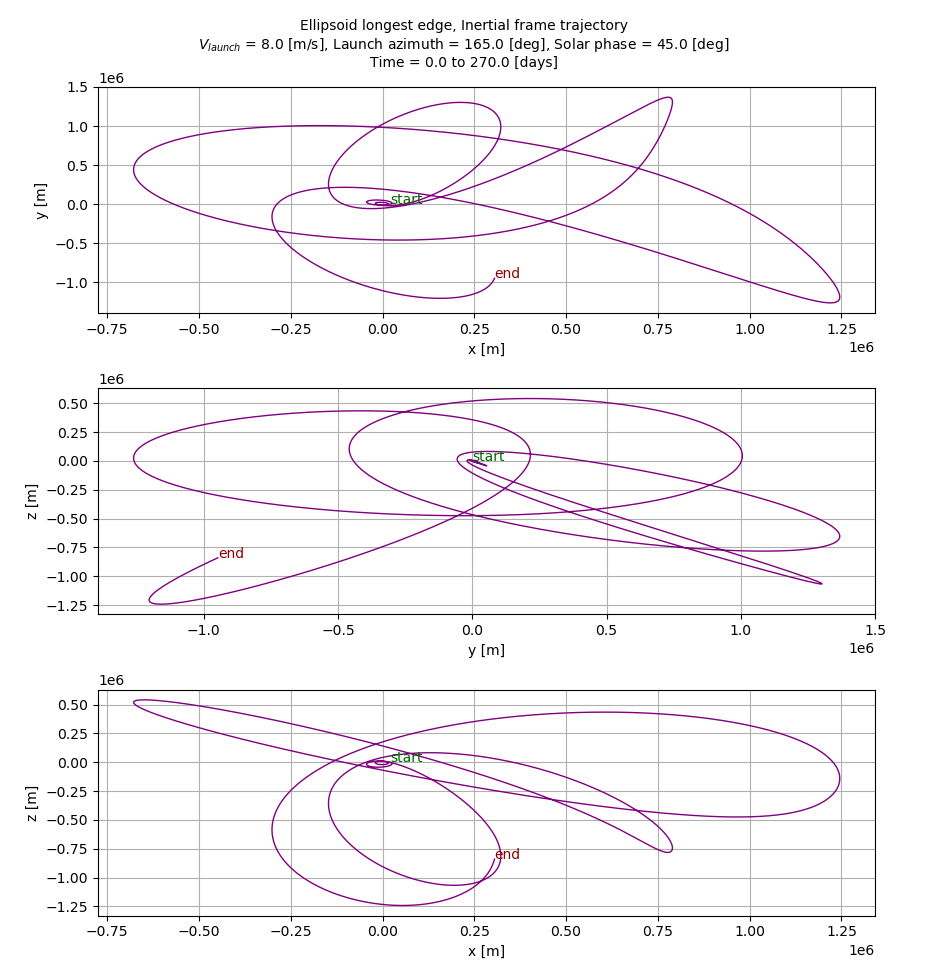
\includegraphics[width=\textwidth, height=\textheight]{longest_edge_perturbations/3.2Density_1cmSize/2dTrajectory_8ms_165Azimuth_45solarPhase_inertialFrame.png}
\caption{2D inertial frame trajectory of capture regolith for case number 8 in \Cref{tab:LoGSP_1_capture}. Particle code LoGSP-1.}
\label{fig:LoGSP_1_capture_case_8_2d_traj_inertialFrame}
\end{figure}
\FloatBarrier
%%%
\begin{figure}[htb]
\centering
\captionsetup{justification=centering}
% another option for includegraphics - keepaspectratio
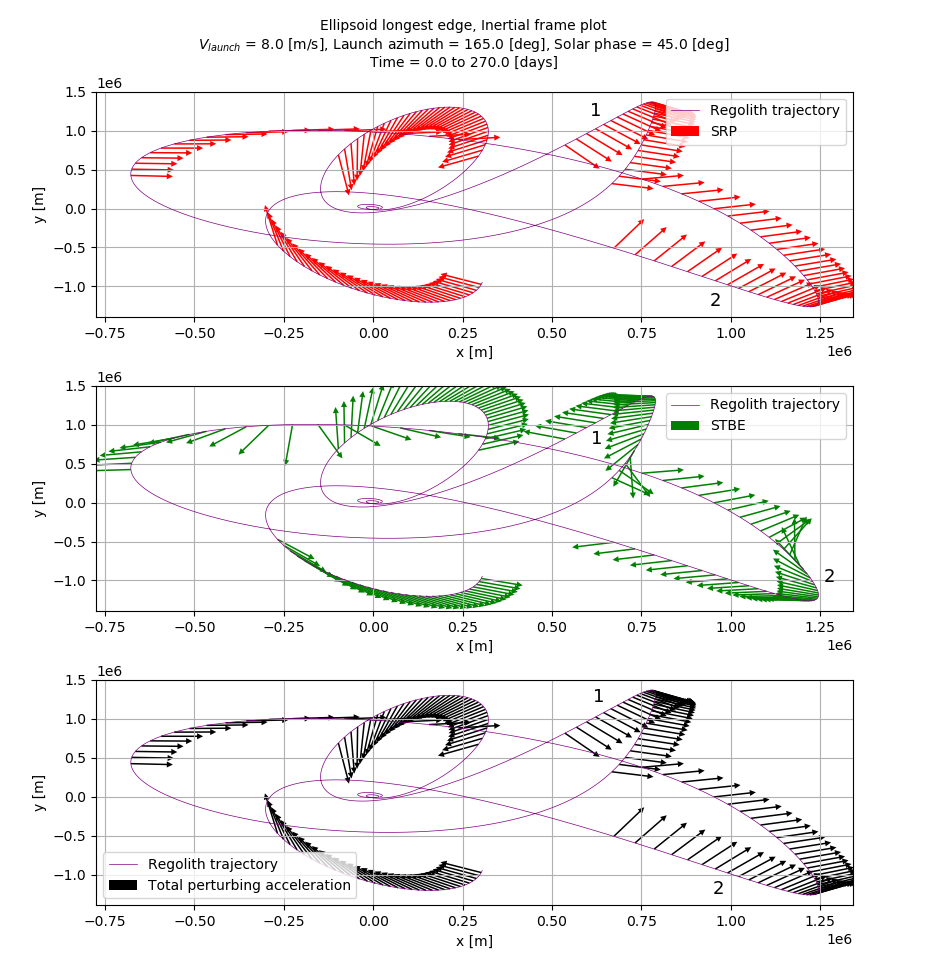
\includegraphics[width=\textwidth, height=\textheight]{longest_edge_perturbations/3.2Density_1cmSize/TotalPerturbingVector_xyPlane_completeTraj_8ms_165DegAzim_45SolarPhase_edit.png}
\caption{2D trajectory of capture regolith for case number 8 in \Cref{tab:LoGSP_1_capture} with direction of \gls{SRP} and \gls{STBE} perturbation vectors along with the sum total of the two. Note that the vectors are shown only for those parts of the trajectory where the \gls{SRP} magnitude is of the same order as that of the asteroid's gravitational acceleration. For those very same points along the trajectory, the magnitude of the \gls{STBE} is always 1.0 order of magnitude smaller than the gravitational acceleration. Particle code LoGSP-1.}
\label{fig:LoGSP_1_capture_case_8_2d_trajectory_perturbationVectors}
\end{figure}
\FloatBarrier
%%%
Let us begin with capture case number 8 in \Cref{tab:LoGSP_1_capture}. \Cref{fig:LoGSP_1_capture_case_8_2d_trajectory_comparative_inertialFrame} shows two different trajectories for the particle launched with the same initial conditions. The one shown in dotted line is for the case when Solar perturbations were omitted from the simulation, which eventually results in the particle escaping the asteroid after 1.4 [days]. The one in the solid line shows the capture trajectory (actually a section of the entire capture trajectory as seen in \Cref{fig:LoGSP_1_capture_case_8_2d_traj_inertialFrame}) when Solar perturbations were included in the simulation. Note that we show the perturbed trajectory (capture case) for the same amount of time (1.4 [days] instead of 270.0 [days]) as taken by the unperturbed trajectory (escape case) to be able to do a one-to-one comparison. The arrows plotted along this trajectory indicate the direction of the perturbing acceleration due to \gls{SRP}. \Cref{fig:LoGSP_1_capture_case_8_2d_trajectory_comparative_animation} directs to an animation for both the unperturbed and perturbed trajectory.
%%%
\begin{figure}[htb]
\centering
\captionsetup{justification=centering}
% another option for includegraphics - keepaspectratio

\includegraphics[scale=0.25]{longest_edge_perturbations/3.2Density_1cmSize/qrcode_comparative_8ms_165Azimuth_45SolarPhase.png}
\caption{2D trajectory animation (XY Plane) of capture regolith for case number 8 in \Cref{tab:LoGSP_1_capture}. Particle code LoGSP-1. Scan the QR code to view the animation or use the following web-link: \url{https://youtu.be/CdFKKR3UDJ0}}
\label{fig:LoGSP_1_capture_case_8_2d_trajectory_comparative_animation}
\end{figure}
\FloatBarrier
%%%
%%%
\begin{figure}[htb]
\centering
\captionsetup{justification=centering}
% another option for includegraphics - keepaspectratio
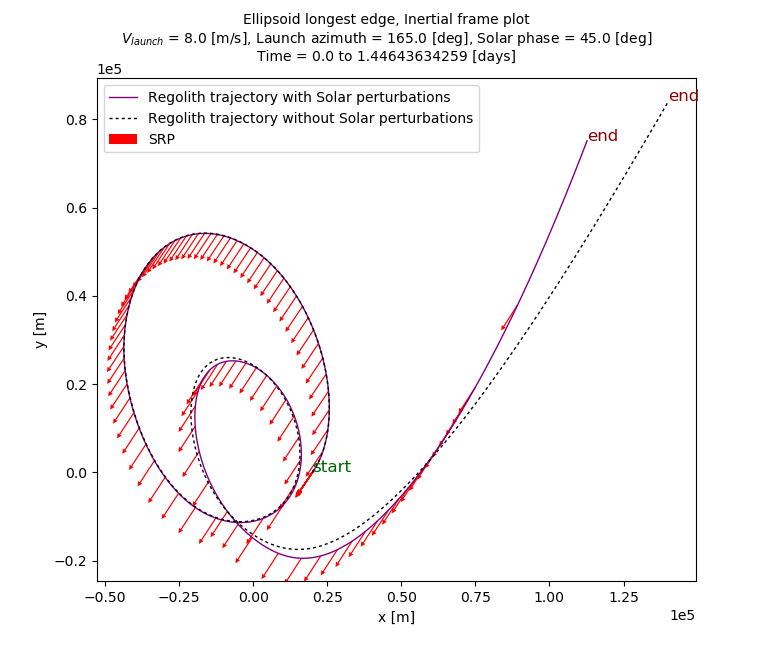
\includegraphics[scale=0.70]{longest_edge_perturbations/3.2Density_1cmSize/singlePlot_comparative_PerturbationVector_8ms_165Azimuth_45SolarPhase_inertialFrame.png}
\caption{Inertial frame 2D trajectory (XY plane) of capture regolith for case number 8 in \Cref{tab:LoGSP_1_capture} with direction of \gls{SRP} perturbation vector compared with the trajectory of a particle launched with the same initial conditions but in absence of Solar perturbations. Particle code LoGSP-1.}
\label{fig:LoGSP_1_capture_case_8_2d_trajectory_comparative_inertialFrame}
\end{figure}
\FloatBarrier
%%%
%%%
\begin{figure}[htb]
\centering
\captionsetup{justification=centering}
% another option for includegraphics - keepaspectratio
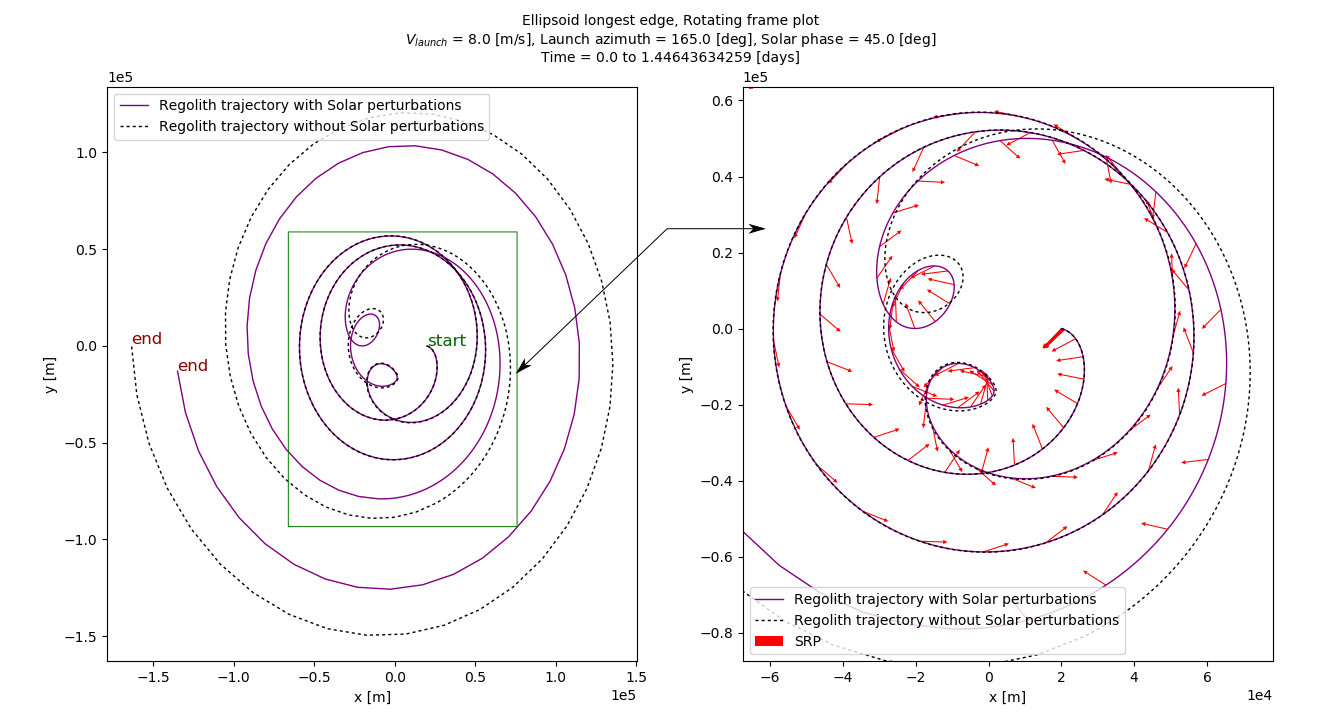
\includegraphics[angle=90, width=\textwidth, height=\textheight]{longest_edge_perturbations/3.2Density_1cmSize/singlePlot_comparative_PerturbationVector_8ms_165Azimuth_45SolarPhase_bodyFrame_edit.png}
\caption{Rotating frame 2D trajectory (XY plane) of capture regolith for case number 8 in \Cref{tab:LoGSP_1_capture} with direction of \gls{SRP} perturbation vector compared with the trajectory of a particle launched with the same initial conditions but in absence of Solar perturbations. Particle code LoGSP-1.}
\label{fig:LoGSP_1_capture_case_8_2d_trajectory_comparative_bodyFrame}
\end{figure}
\FloatBarrier
%%%
From the animation we can see that even as the particle has just been lofted from the surface of the asteroid, there are very subtle and minute differences, in the range to the particle and its velocity, between the perturbed and unperturbed trajectory. Ofcourse as the state vector differences are so small initially, the perturbed and unperturbed trajectory overlap with each other and can be seen so in \Cref{fig:LoGSP_1_capture_case_8_2d_trajectory_comparative_inertialFrame}. Later, as the trajectory progresses, we see that these differences increase to a significant quotient because the effect of \gls{SRP} adds up after a certain amount of time. A snippet from the trajectory animation in \Cref{fig:LoGSP_1_capture_case_8_2d_comparative_animation_snippet} clearly shows the said differences. This snippet was taken around the moment when the perturbed and unperturbed trajectory start to separate from each other.
%%%
\begin{figure}[htb]
\centering
\captionsetup{justification=centering}
% another option for includegraphics - keepaspectratio
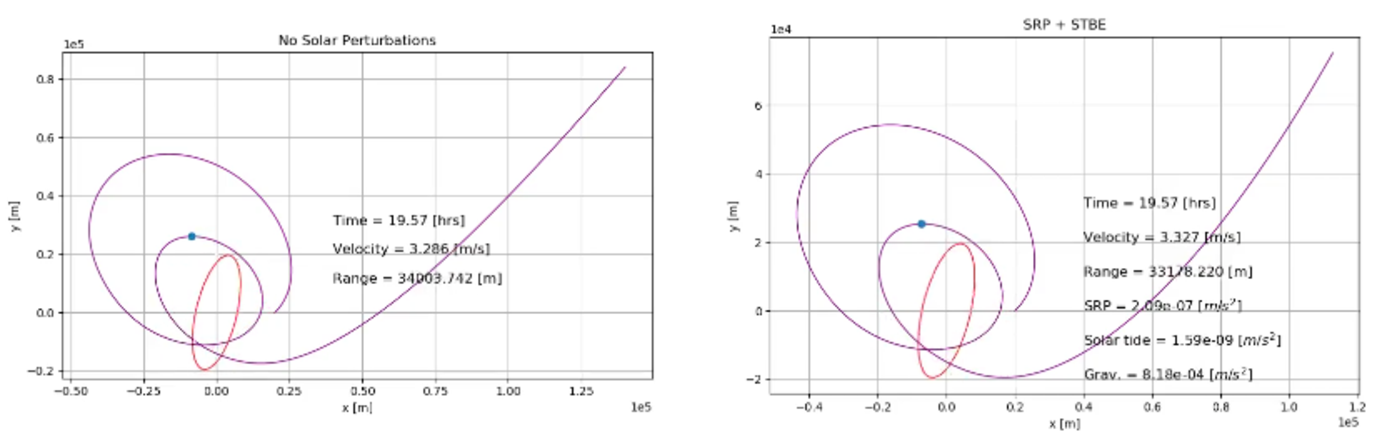
\includegraphics[width=\textwidth]{longest_edge_perturbations/3.2Density_1cmSize/animation_snippet_8ms_165Azimuth_45SolarPhase_comparative_xyTraj.pdf}
\caption{Animation snippet of the inertial frame 2D trajectory (XY plane) of capture regolith for case number 8 in \Cref{tab:LoGSP_1_capture}. The trajectory on the left is for the case when Solar perturbations were omitted from the simulation and the trajectory on the right includes them. Note the differences in the range to the particle and its velocity for the same time stamp and rotational state of the asteroid. Particle code LoGSP-1.}
\label{fig:LoGSP_1_capture_case_8_2d_comparative_animation_snippet}
\end{figure}
\FloatBarrier
%%%
In \Cref{fig:LoGSP_1_capture_case_8_2d_trajectory_comparative_inertialFrame} we can see that the departure in the perturbed trajectory from the unperturbed one is consistent with the direction in which the perturbing acceleration from \gls{SRP} is acting. This can also be seen a bit more clearly when we look at the trajectory plot in the asteroid centric rotating frame or the body frame as shown in \Cref{fig:LoGSP_1_capture_case_8_2d_trajectory_comparative_bodyFrame}. The plot on the left shows the trajectory for 1.4 [days] (i.e. until escape for the unperturbed trajectory) as viewed from the rotating frame, and the plot on the right zooms into a small part of this trajectory to show how \gls{SRP} is responsible for changing the course of the particle. It is easily seen how the \gls{SRP} vector pulls the trajectory away from the unperturbed one, thereby avoiding an escape scenario.


Note that we have not shown the direction for perturbing acceleration due to \gls{STBE} because its magnitude was 5.0 orders smaller than the gravitational acceleration for when the particle is close to the asteroid, which it is in the plots shown in \Cref{fig:LoGSP_1_capture_case_8_2d_trajectory_comparative_inertialFrame} and \Cref{fig:LoGSP_1_capture_case_8_2d_trajectory_comparative_bodyFrame}. The magnitude of acceleration due to \gls{SRP} is however 3.0 orders smaller than the gravitational acceleration. But, as we saw earlier, it induces small changes in the state vector of the particle which eventually builds up as the trajectory progresses and then eventually leads to a capture scenario. Ofcourse \gls{SRP} is not the sole criterion here to get a capture orbit, and we will see it shortly, that inclusion of \gls{SRP} results in a situation where the regolith/particle has a different phasing (in this context we mean the location of the particle with respect to a rotating asteroid) compared to its unperturbed counterpart which leads to the particle getting trapped around the asteroid.


%\bibliographystyle{bibgen}
%\bibliography{report22}
%\bibliography{report22.bib}{}
\printbibliography[heading=bibintoc]

\begin{appendices}
\addtocontents{toc}{\protect\setcounter{tocdepth}{0}}
  \chapter{Extra Figures}
  This appendix contains figures which are used to support the explanation of certain results, arguments and conclusions in the main part of the Thesis report.
    %%%
    \begin{figure}[htb]
    \centering
    \captionsetup{justification=centering}
    % another option for includegraphics - keepaspectratio
    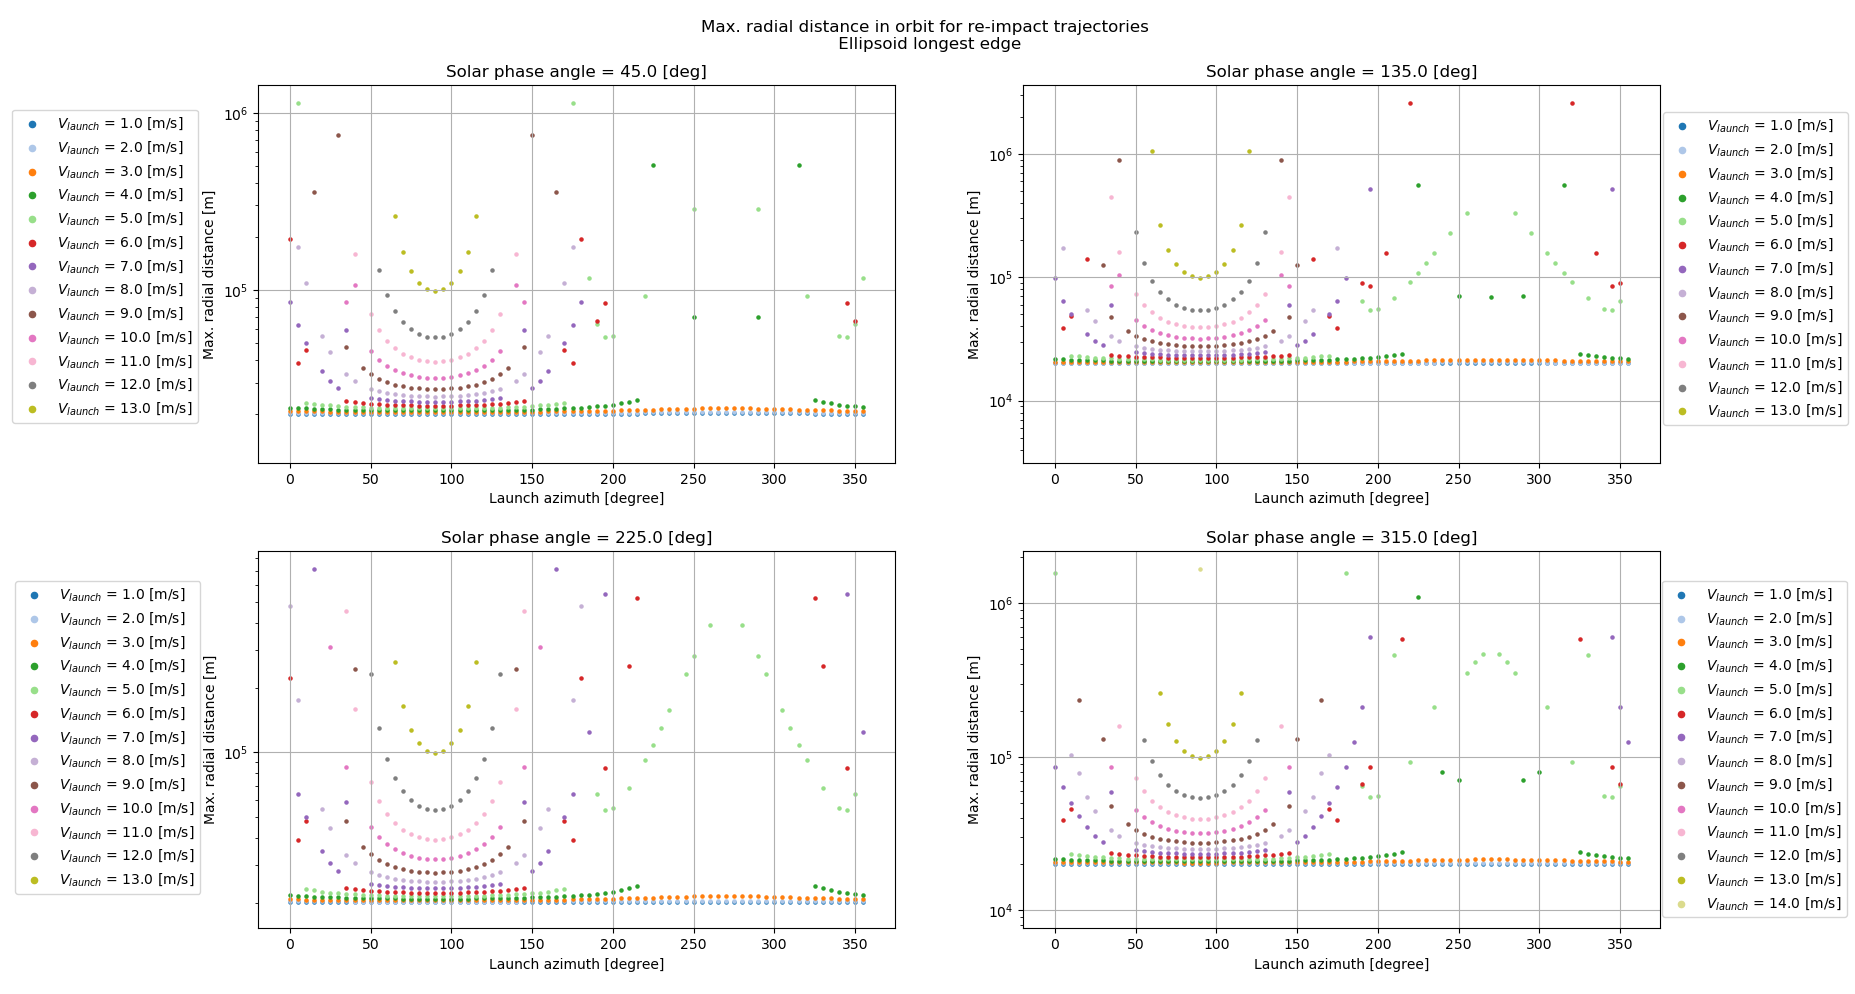
\includegraphics[angle=90, width=\textwidth, height=\textheight]{Results/Images/longest_edge_perturbations/3.2Density_1cmSize/maxAltitude_reimpactCase.png}
    \caption{Maximum radial distance (from the centre of the asteroid) attained by the regolith in orbit for different launch velocities and launch azimuths. The particles were launched from the longest edge of the ellipsoid (asteroid). Plots are for particle code LoGSP-1 and only for the re-impact scenario.}
    \label{fig:LoGSP_1_maxAltitude_reimpactscenario}
    \end{figure}
    \FloatBarrier
    %%%
    %%%
    \begin{figure}[htb]
    \centering
    \captionsetup{justification=centering}
    % another option for includegraphics - keepaspectratio
    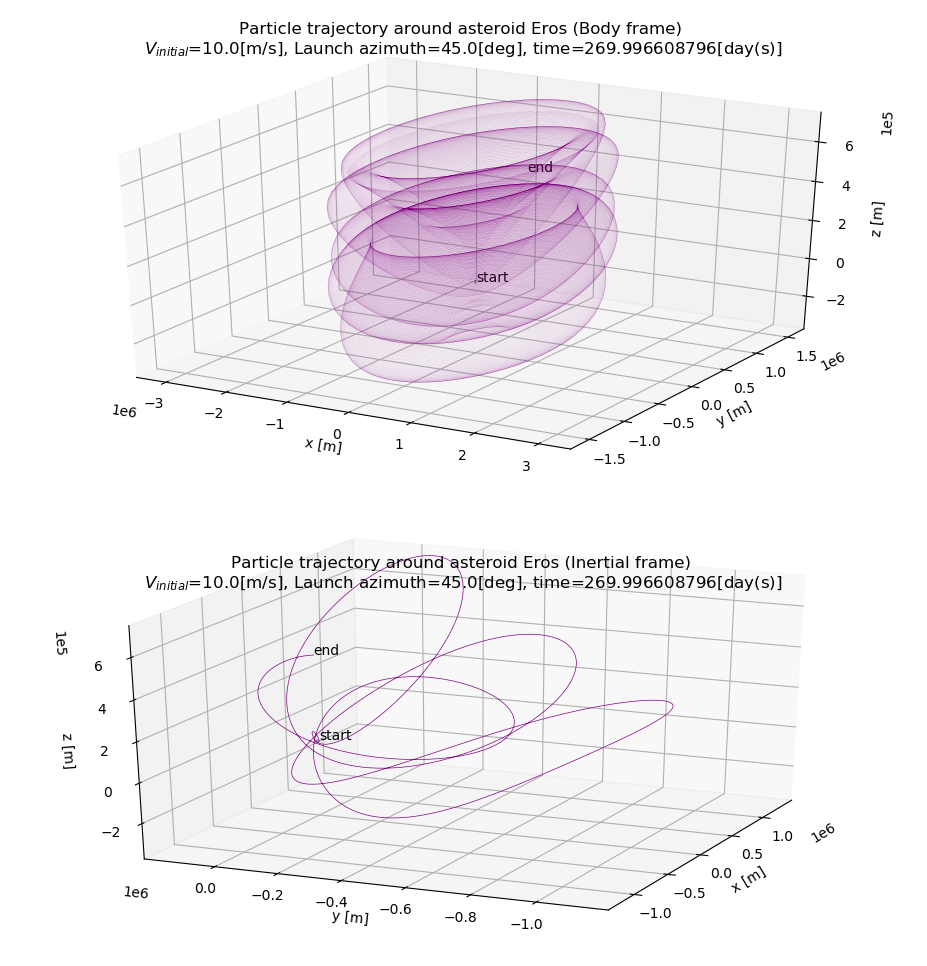
\includegraphics[width=\textwidth, height=\textheight]{Results/Images/longest_edge_perturbations/3.2Density_1cmSize/3dTrajectory_10ms_45Azimuth_315solarPhase.png}
    \caption{3D trajectory of capture regolith for case number 5 in \Cref{tab:LoGSP_1_capture}. Particle code LoGSP-1.}
    \label{fig:LoGSP_1_capture_case_5_3d_trajectory}
    \end{figure}
    \FloatBarrier
    %%%
    %%%
    \begin{figure}[htb]
    \centering
    \captionsetup{justification=centering}
    % another option for includegraphics - keepaspectratio
    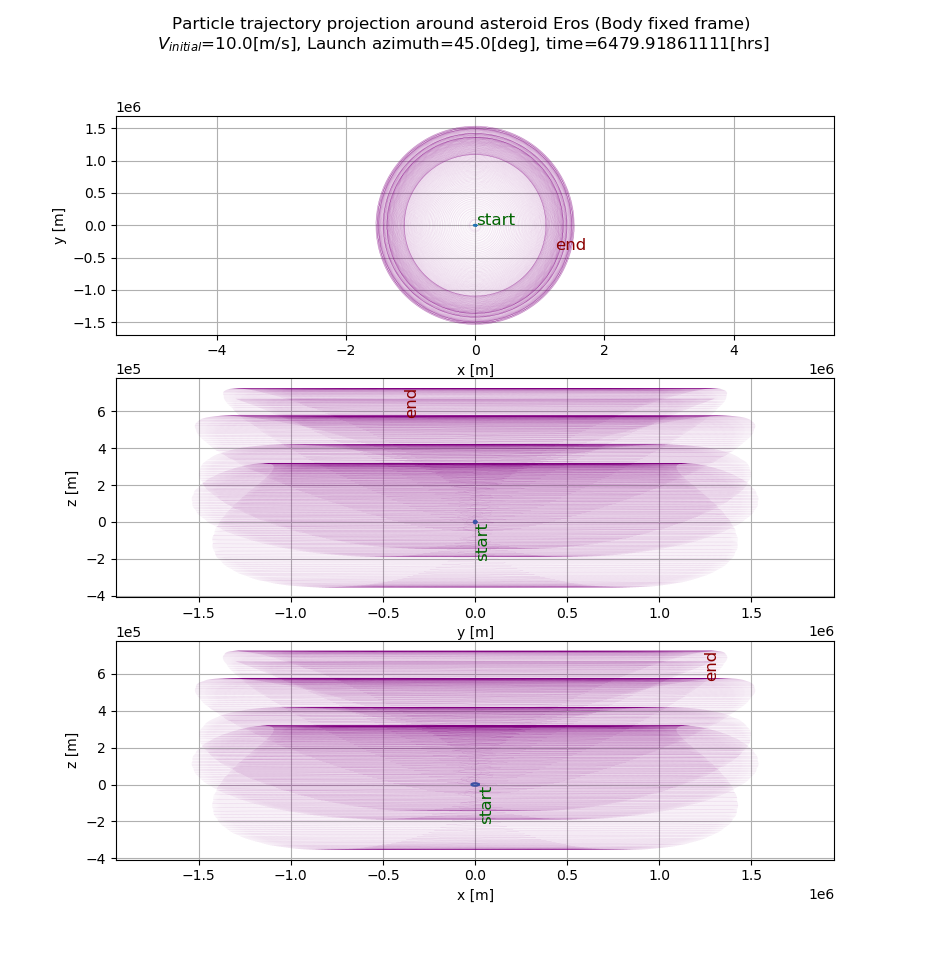
\includegraphics[width=\textwidth, height=\textheight]{Results/Images/longest_edge_perturbations/3.2Density_1cmSize/2dTrajectory_10ms_45Azimuth_315solarPhase_bodyFrame.png}
    \caption{2D rotating frame trajectory of capture regolith for case number 5 in \Cref{tab:LoGSP_1_capture}. Particle code LoGSP-1.}
    \label{fig:LoGSP_1_capture_case_5_2d_traj_bodyFrame}
    \end{figure}
    \FloatBarrier
    %%%
    %%%
    \begin{figure}[htb]
    \centering
    \captionsetup{justification=centering}
    % another option for includegraphics - keepaspectratio
    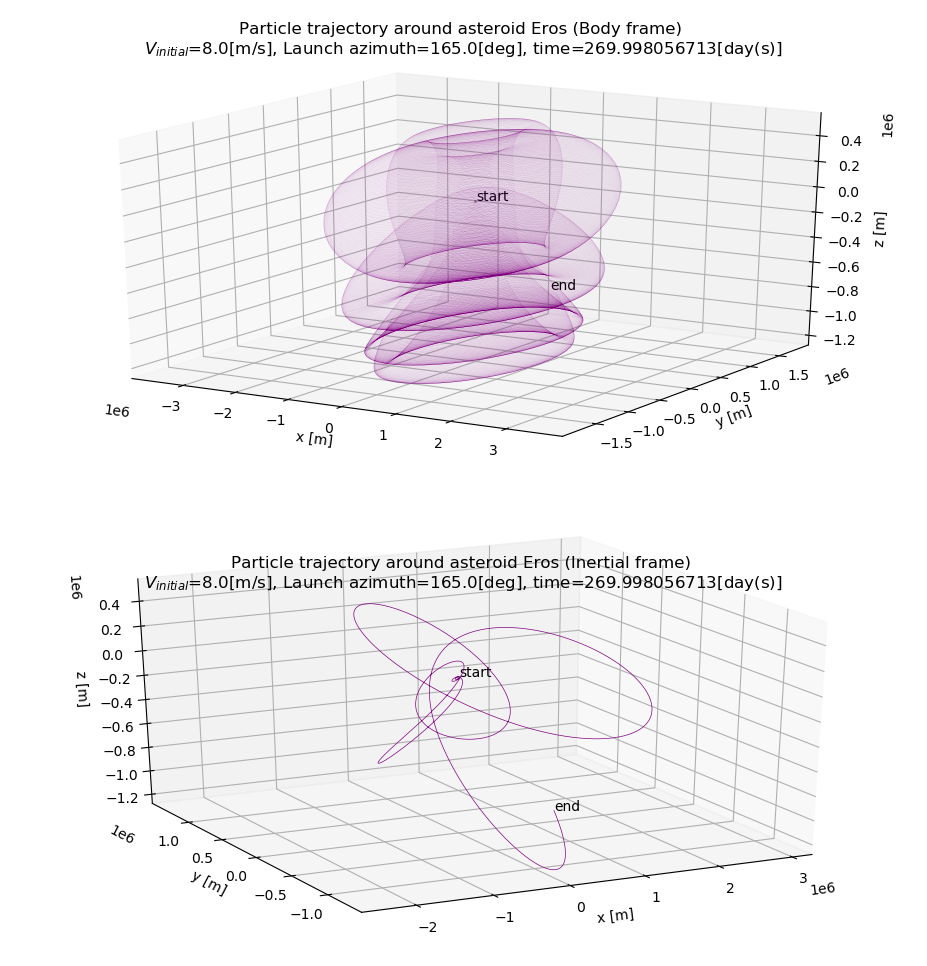
\includegraphics[width=\textwidth, height=\textheight]{Results/Images/longest_edge_perturbations/3.2Density_1cmSize/3dTrajectory_8ms_165Azimuth_45solarPhase.png}
    \caption{3D trajectory of capture regolith for case number 5 in \Cref{tab:LoGSP_1_capture}. Particle code LoGSP-1.}
    \label{fig:LoGSP_1_capture_case_8_3d_trajectory}
    \end{figure}
    \FloatBarrier
    %%%
    %%%
    \begin{figure}[htb]
    \centering
    \captionsetup{justification=centering}
    % another option for includegraphics - keepaspectratio
    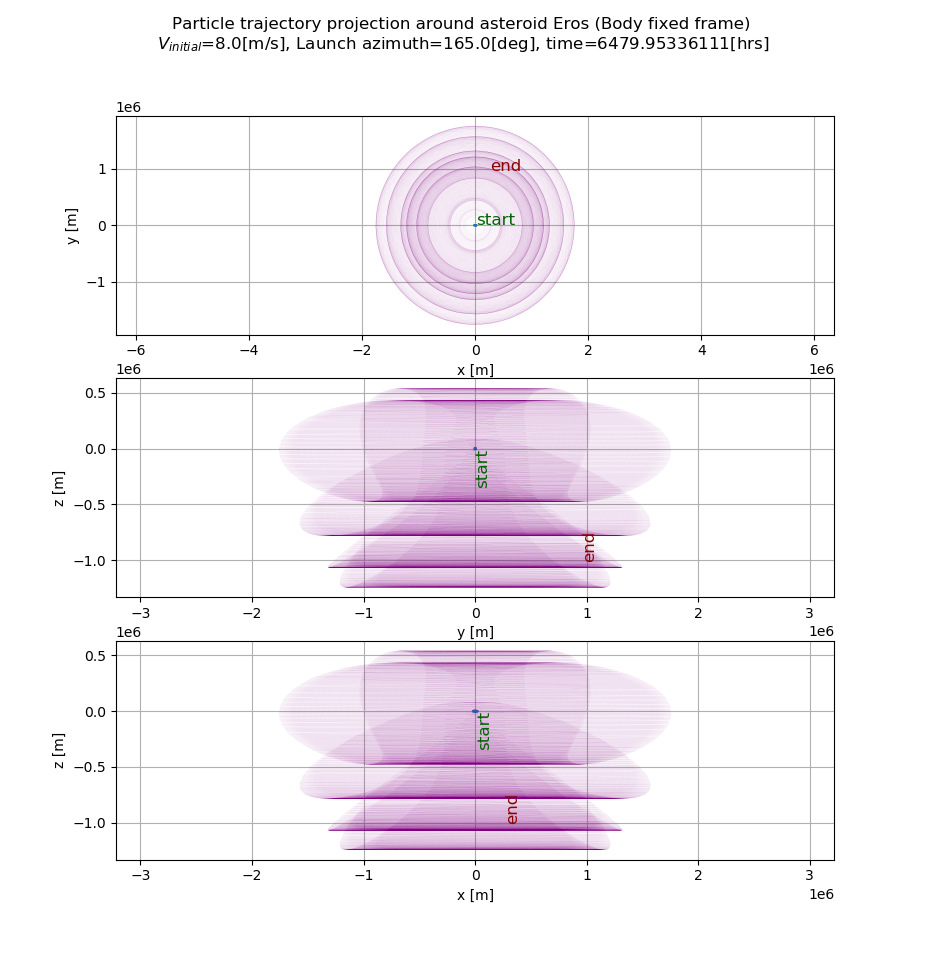
\includegraphics[width=\textwidth, height=\textheight]{Results/Images/longest_edge_perturbations/3.2Density_1cmSize/2dTrajectory_8ms_165Azimuth_45solarPhase_bodyFrame.png}
    \caption{2D rotating frame trajectory of capture regolith for case number 8 in \Cref{tab:LoGSP_1_capture}. Particle code LoGSP-1.}
    \label{fig:LoGSP_1_capture_case_8_2d_traj_bodyFrame}
    \end{figure}
    \FloatBarrier
    %%%
\end{appendices}

\end{document}
